\documentclass[12pt,a4paper]{report}

% ---------- PACKAGES ----------
\usepackage[a4paper,margin=1in]{geometry}
\usepackage{graphicx}
\usepackage{booktabs}
\usepackage{longtable}
\usepackage{array}
\usepackage{ragged2e}

\usepackage{enumitem}
\usepackage{hyperref}
\usepackage{caption}
\usepackage{amsmath}
\usepackage{setspace}
\usepackage{fancyhdr}
\usepackage[compact]{titlesec}
\usepackage[htt]{hyphenat}   % permit hyphenation inside \texttt{...}

% Long \texttt{} identifiers (e.g. PREFERENCE\_PROFILE) cannot be broken by
% default and overflow the margin; this lets TeX stretch a line instead.
\setlength{\emergencystretch}{3em}

% ---------- COMPACT SPACING ----------
\titlespacing*{\chapter}{0pt}{-20pt}{10pt}
\titlespacing*{\section}{0pt}{10pt}{4pt}
\titlespacing*{\subsection}{0pt}{8pt}{3pt}
\setlength{\parskip}{4pt}
\setlength{\textfloatsep}{20pt plus 4pt minus 4pt}
\setlength{\intextsep}{18pt plus 4pt minus 4pt}
\setlength{\abovecaptionskip}{10pt}
\setlength{\belowcaptionskip}{14pt}

% ---------- HYPERLINK / TOC SETUP ----------
\hypersetup{
    colorlinks=true,
    linkcolor=black,
    urlcolor=blue,
    citecolor=black,
    bookmarksopen=true,
    pdftitle={System Design Document (SDD) - COHAB},
    pdfauthor={ Puranjyoti Bera, Alwin N Joseph}
}

% ---------- HEADER/FOOTER ----------
\pagestyle{fancy}
\fancyhf{}
\fancyfoot[C]{\thepage}

% ---------- CUSTOM COLUMN TYPE FOR TABLES ----------
\newcolumntype{L}[1]{>{\raggedright\arraybackslash}p{#1}}

\title{\textbf{System Design Document (SDD)}\\[0.5em]
COHAB -- A Compatibility-Based Roommate Matching Platform}
\author{Puranjyoti Bera (2548035) and Alwin N Joseph (2548006)\\[1em]
Under the guidance of\\
Dr Sathya P}
\date{5\textsuperscript{th} July 2026}

\begin{document}

% ---------------- TITLE PAGE ----------------
\begin{titlepage}
    \centering
    
\includegraphics[width=0.9\textwidth]{images/image1.png}\\[2em]
\vspace{25mm}
    {\LARGE \textbf{System Design Document (SDD)}}\\[1em]
\vspace{10mm}
    {\Large \textbf{COHAB -- A Compatibility-Based Roommate}}\\[3em]
\vspace{-5mm}
    {\Large \textbf{Matching Platform}}\\[3em]
\vspace{10mm}
    by\\[0.5em]
    {\large Alwin N Joseph (2548006) and Puranjyoti Bera (2548035)}\\[2em]

    Under the guidance of\\[0.5em]
    {\large Dr. Sathya P}\\[3em]

    {\large \textbf{5\textsuperscript{th} July 2026}}

\end{titlepage}

% ---------------- TABLE OF CONTENTS ----------------
\tableofcontents
\clearpage

% ---------------- LIST OF FIGURES ----------------
\listoffigures
\clearpage

% ==================================================================
\chapter{Introduction to System Design}

\section{Purpose}

Cohab is a compatibility-based roommate matching platform designed to replace the informal, unverified way people use to currently find roommate like through referrals, Telegram groups, and generic classifieds with a structured, data-driven matching process. Traditional roommate search leaves large gaps in verification and provides no structured way to compare lifestyle expectations before move-in, which tends to surface later as disputes, early move-outs, and occasionally unsafe living situations.

The proposed system captures a verified user profile and a structured lifestyle questionnaire, computes a weighted compatibility score between users using statistical and semantic similarity measures, and returns a ranked, explainable match list. A moderated in-app chat allows matched users to communicate before sharing personal contact information or meeting in person. Outcomes from accepted and rejected matches are logged and periodically used to refine the scoring weights, so the matching engine improves with real usage rather than remaining fixed at its initial, expert-assigned configuration.

This System Design Document (SDD) translates the requirements identified during the Requirement Analysis and SRS phases into a detailed technical design covering architecture, workflows, database design, interaction models, algorithms, and interface specifications. The document serves as a blueprint for the implementation, testing, and deployment phases of the project.

\vspace{10mm}
\section{Scope of this Document}

The scope of this document is limited to the design aspects of Cohab and includes the major architectural, functional, and technical decisions required for implementation. The document covers:

\begin{itemize}[noitemsep]
    \item System Architecture (layered view of the platform)
    \vspace{1mm}
    \item Component Diagram
    \vspace{1mm}
    \item Data Flow Diagrams (Level 0 and Level 1)
    \vspace{1mm}
    \item Use Case Diagram
    \vspace{1mm}
    \item Entity Relationship Diagram (ERD) and Data Dictionary
    \vspace{1mm}
    \item Class Diagram
    \vspace{1mm}
    \item Activity Diagram
    \vspace{1mm}
    \item Sequence Diagram (core matching workflow)
    \vspace{1mm}
    \item Algorithms and Data Structures
    \vspace{1mm}
    \item Security, Privacy and Data Protection Design
    \vspace{1mm}
    \item Evaluation Design and Success Metrics
    \vspace{1mm}
    \item Interface Design (key screens)
    \vspace{1mm}
    \item Gantt Chart and PERT/CPM Network (project schedule)
\end{itemize}

\section{Design Objectives}

The primary objectives of the system design are:

\begin{itemize}[noitemsep]
    \item Reduce the manual effort and uncertainty involved in finding a compatible roommate.
    \vspace{1mm}
    \item Improve match quality and trust through verified profiles and explainable compatibility scores.
    \vspace{1mm}
    \item Keep students in control of the final decision --- the system ranks and explains candidates but never auto-assigns a roommate without mutual consent.
    \vspace{1mm}
    \item Support modularity and scalability so new modules (e.g. group matching, operator integrations) can be added without modifying existing matching logic.
    \vspace{1mm}
    \item Ensure maintainability through separation of concerns and a layered architecture.
    \vspace{1mm}
    \item Provide explainable compatibility recommendations to improve user trust in the system.
    \vspace{1mm}
    \item Build in a feedback loop so scoring weights improve from real usage data over time rather than staying fixed.
    \vspace{1mm}
    \item Separate non-negotiable requirements from graded preferences, so that a numerically high compatibility score can never be produced for a candidate who is infeasible in practice.
    \vspace{1mm}
    \item Treat safety and identity verification as first-class design concerns rather than as after-the-fact moderation, and make every account action auditable.
    \vspace{1mm}
    \item Collect, store and process personal data in a manner consistent with the SRS Data Privacy requirement and the Digital Personal Data Protection (DPDP) Act, 2023, including purpose limitation, retention limits and the right to erasure.
\end{itemize}

% ==================================================================
\chapter{System Architecture}

\section{Overview}

Cohab follows a layered, modular architecture consisting of a presentation layer (responsive web portal / mobile-responsive UI), an API gateway and orchestration layer, an application / business-logic layer (FastAPI services), an AI/ML \& integration layer (scikit-learn, sentence-transformers, pandas/NumPy, and an SMTP/SMS notifier), and a persistence layer (PostgreSQL, MongoDB, Redis and a restricted object store). This separation allows each layer to evolve independently, satisfying the Modifiability and Reusability non-functional requirements defined in the SRS.

The API gateway layer is drawn explicitly because orchestration is a server-side responsibility. The client issues intent-level requests (``score my profile against the pool'', ``open a chat with this match'') and the gateway sequences the underlying service calls; the browser is never trusted to compose a business workflow, because a client that orchestrates can also be modified to skip steps such as verification checks, consent capture or rate limiting.

\vspace{3.5mm}
\begin{figure}[htbp]
    \centering
    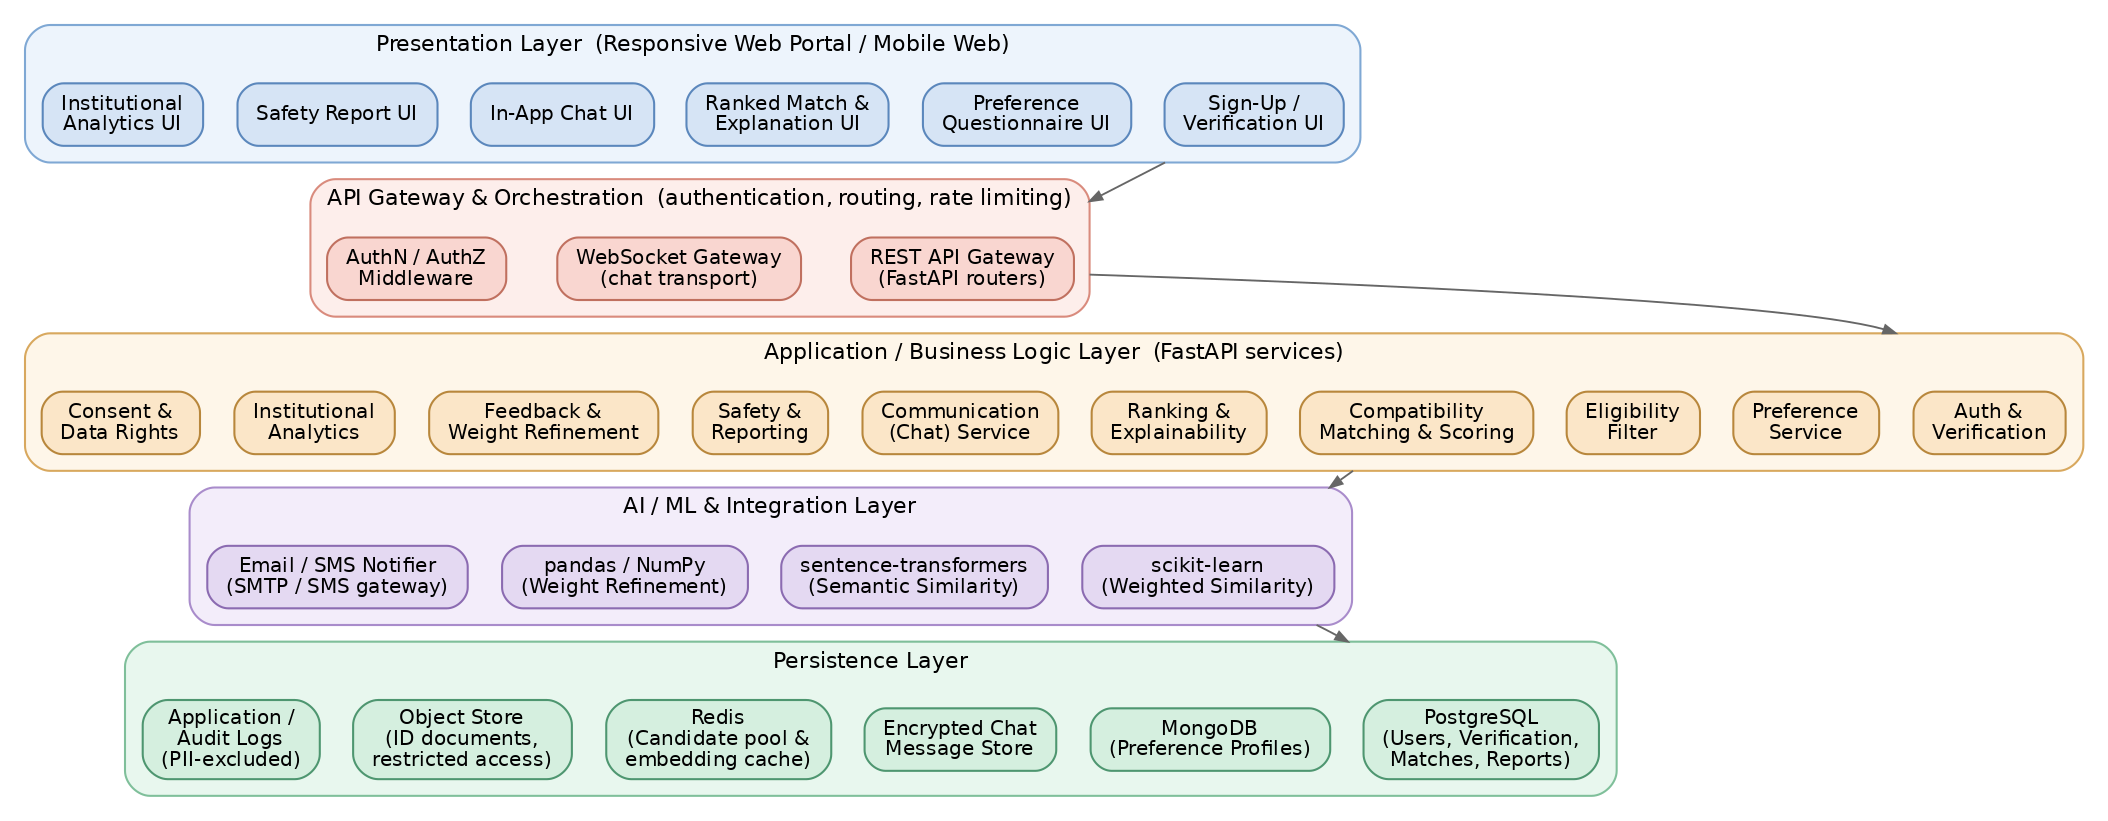
\includegraphics[width=1.0\textwidth]{images/image2.png}
    \caption{Layered System Architecture of Cohab}
    \label{fig:2.1}
\end{figure}

As shown in Figure \ref{fig:2.1}, the presentation layer provides interfaces for students to sign up and verify their identity, complete the preference questionnaire, review ranked and explainable matches, chat with matched users, file safety reports, and --- for institutional partners --- view usage analytics. The gateway layer authenticates every request, enforces rate limits and routes traffic to the appropriate service. The application layer coordinates authentication and verification, preference storage, eligibility filtering, compatibility matching and scoring, ranking and explainability, in-app communication, safety and reporting, feedback-driven weight refinement, institutional analytics, and consent and data-rights handling. The AI/ML layer performs weighted similarity scoring and semantic similarity computation on free-text profile fields, aggregates match-outcome feedback for periodic weight refinement, and dispatches email/SMS notifications. The persistence layer stores structured relational data in PostgreSQL, evolving preference-profile documents in MongoDB, cached candidate pools and precomputed embeddings in Redis, encrypted chat messages in a dedicated message store, and identity documents in a restricted object store, while excluding personal data from application and audit logs.

\section{Layer Description}

\textbf{Presentation Layer:} a responsive, multi-page web application (mobile-responsive) providing sign-up/verification, preference questionnaire, ranked-match and explanation, in-app chat, safety-report, and institutional analytics screens.

\vspace{2mm}
\textbf{API Gateway \& Orchestration Layer:} FastAPI routers terminate all client traffic. Authentication and authorisation middleware validates the session token and the caller's verification status before any business service is reached; per-endpoint rate limits protect the messaging and reporting endpoints from abuse. A separate WebSocket gateway carries in-app chat, since a request/response REST endpoint cannot deliver messages to a connected peer without polling. Business workflows are sequenced here rather than in the browser.

\vspace{2mm}
\textbf{Application Layer:} FastAPI services exposing REST endpoints consumed by the gateway and, per the SRS integration scope, by external college-administration and PG/co-living-operator systems.

\vspace{2mm}
\textbf{AI/ML \& Integration Layer:} scikit-learn performs weighted, rule-based similarity scoring across structured attributes; sentence-transformers compute semantic similarity for free-text profile fields (e.g. lifestyle notes); pandas/NumPy aggregate match-outcome feedback and periodically recompute attribute weights; the email/SMS notifier dispatches match alerts, offline chat notifications, and report-status updates.

\vspace{2mm}
\textbf{Persistence Layer:} PostgreSQL stores Users, Verification Records, Match Scores, Weight Sets, Reports, Consent Records and Feedback, where referential integrity and auditability matter. MongoDB stores the Preference Profile \emph{document}, whose shape is expected to change as the questionnaire is refined. Redis caches eligible candidate pools and precomputed lifestyle-note embeddings. A dedicated store retains encrypted chat messages; identity documents are held in a separate object store with restricted access and a scheduled purge; application and audit logs exclude personal data (PII) per the SRS Data Privacy requirement and India's DPDP Act, 2023.

\vspace{2mm}
\textbf{Reconciling the relational and document stores.} Chapter 6 models \texttt{PREFERENCE\_PROFILE} as a relational table while this chapter places preference profiles in MongoDB; the two are complementary rather than contradictory. The relational table holds the \emph{filterable projection} --- the small, stable set of attributes the eligibility filter and analytics queries must join and index on (city, budget bounds, move-in date, and the categorical lifestyle attributes) --- together with \texttt{profile\_doc\_id}, a reference to the MongoDB document. The document holds the full questionnaire response, including any newly added questions that have not yet been promoted into the relational projection. Promotion of a new attribute into the relational schema is therefore an explicit, versioned migration rather than an implicit schema drift, and the questionnaire can be extended between releases without a database migration blocking it.

% ==================================================================
\chapter{Component Diagram}

\section{Component View of the System}

The component diagram provides a modular view of Cohab and illustrates how the major software components interact with each other. The frontend communicates with a single API gateway component, which routes to the business-logic components; those in turn coordinate AI/ML services and database operations.

\vspace{4mm}
\begin{figure}[htbp]
    \centering
    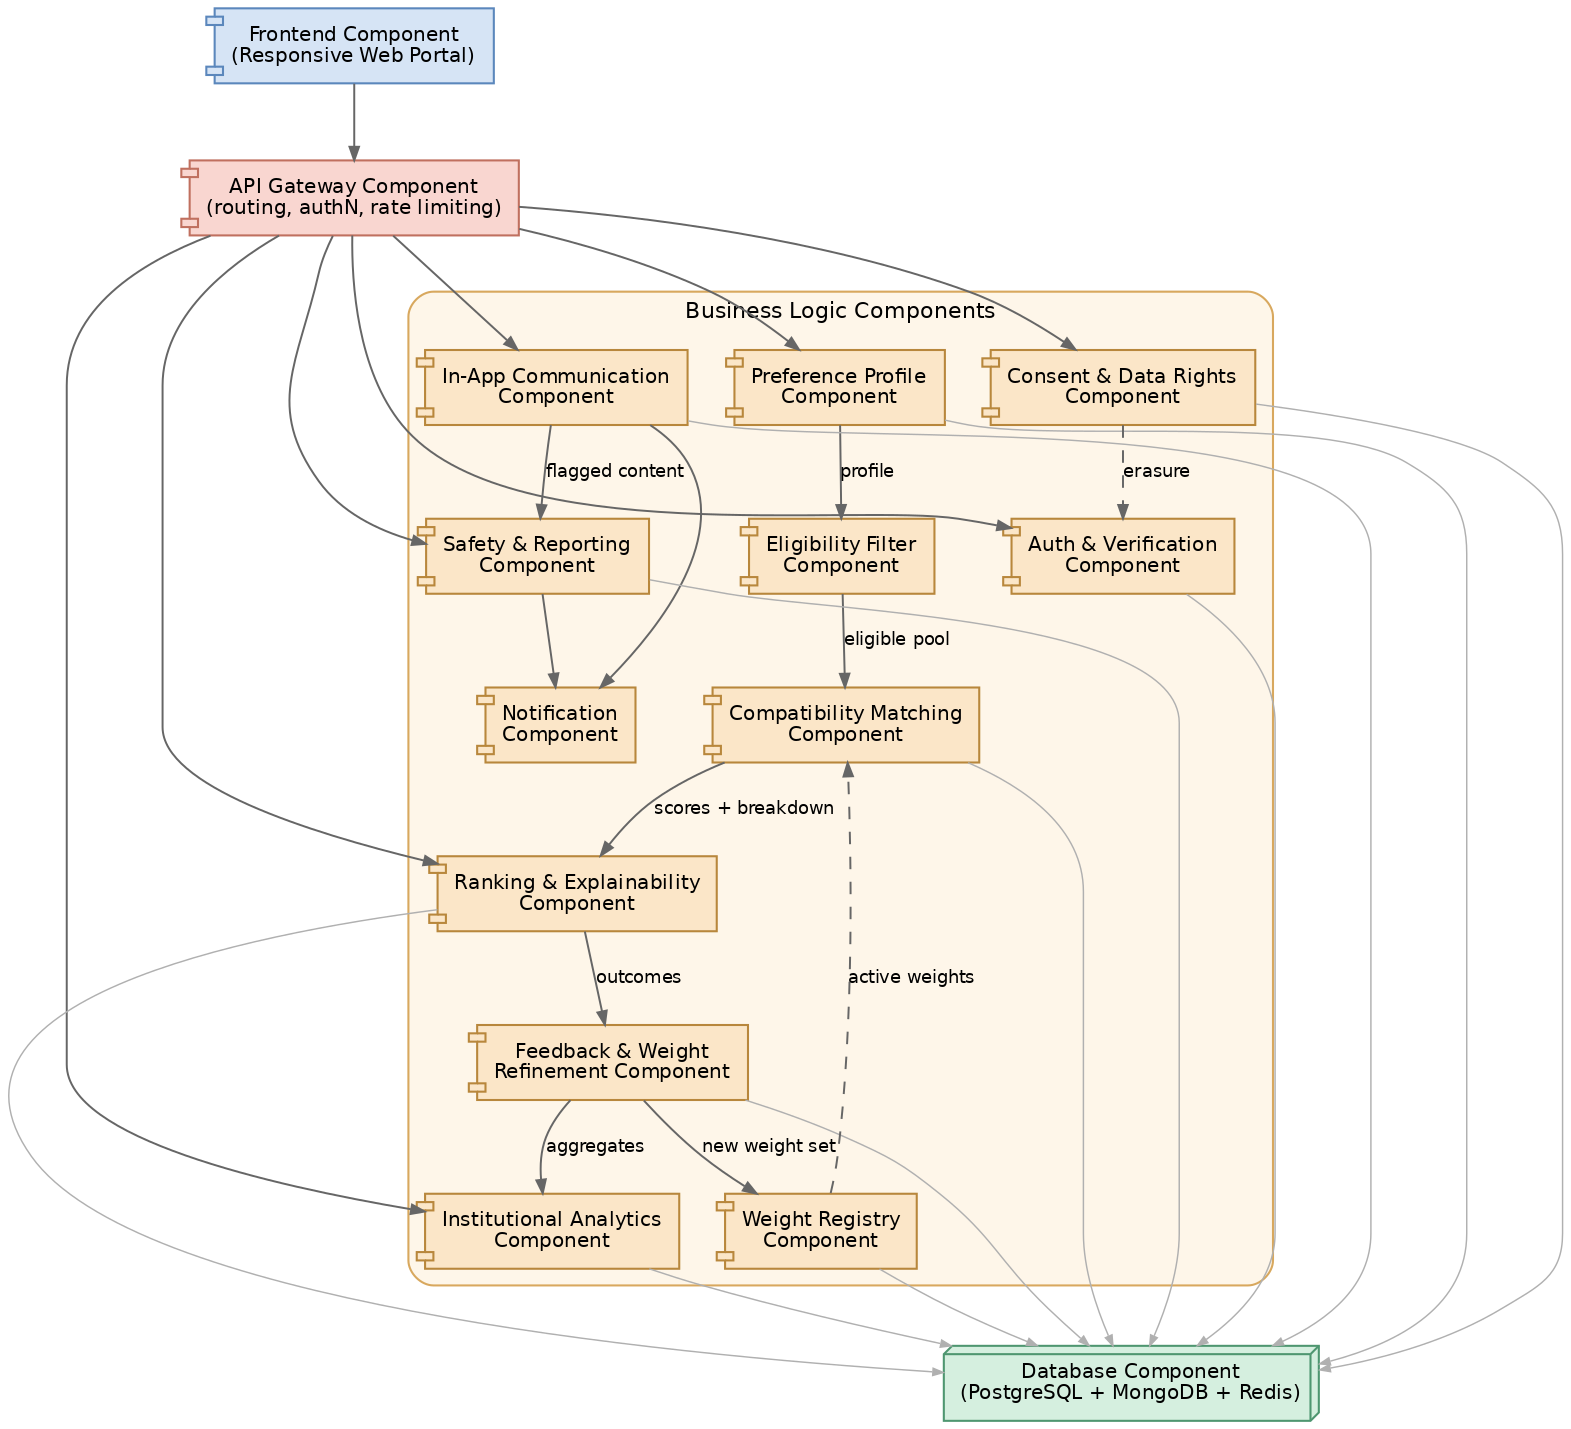
\includegraphics[width=1.0\textwidth]{images/image3.png}
    \caption{Component Diagram of Cohab}
    \label{fig:3.1}
\end{figure}

Figure \ref{fig:3.1} illustrates the modular structure of the proposed system. The web/mobile frontend is a presentation component only: it renders state and captures input, and every request it makes passes through the API Gateway Component, which performs authentication, authorisation and rate limiting before dispatching to a business-logic component. Orchestration therefore lives on the server side, where it can be enforced.

The business-logic tier comprises the Auth \& Verification, Preference Profile, Eligibility Filter, Compatibility Matching, Ranking \& Explainability, In-App Communication, Safety \& Reporting, Feedback \& Weight Refinement, Weight Registry, Notification, Institutional Analytics, and Consent \& Data Rights components. The Preference Profile component supplies both the scored attributes and the user's declared hard constraints to the Eligibility Filter, which reduces the candidate pool before any scoring work is done. The Compatibility Matching component then computes attribute-level similarity scores for that reduced pool, drawing its active weight vector from the Weight Registry component. The Ranking \& Explainability component consumes those scores to produce the ranked, explainable match list and forwards observed outcomes to the Feedback \& Weight Refinement component, which periodically recomputes attribute weights and publishes them back to the Weight Registry as a new, versioned weight set. Routing the refinement loop through the registry rather than directly into the matcher keeps the dependency acyclic and makes it possible to reproduce any historical explanation. The Chat and Safety \& Reporting components both route through the shared Notification component for email/SMS delivery, and the Consent \& Data Rights component drives account erasure and suspension through Auth \& Verification. All components persist and retrieve data through the shared Database Component (PostgreSQL + MongoDB + Redis).

% ==================================================================
\chapter{Data Flow Diagrams}

\section{DFD Level 0 (Context Diagram)}

The context diagram treats the entire system as a single process and shows its interaction with external entities: the Student User, the Matched Roommate Candidate, the Institutional Partner (campus or PG/co-living operator), and the Safety/Moderation Team.
\vspace{4mm}
\begin{figure}[htbp]
    \centering
    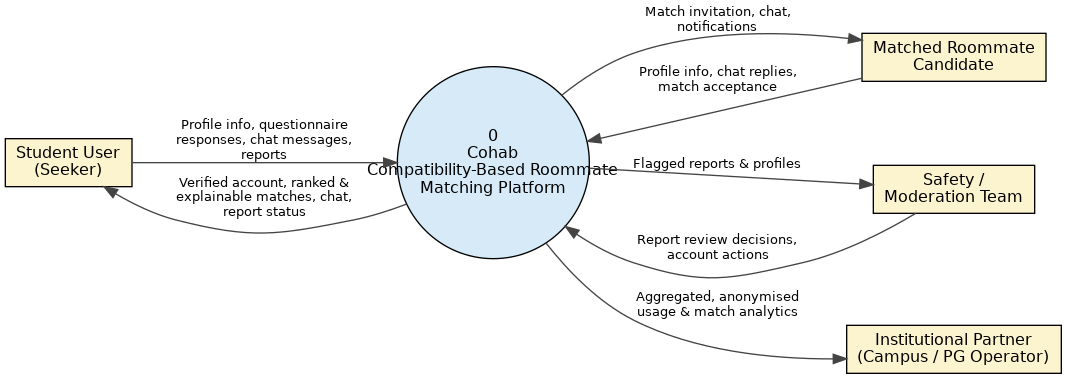
\includegraphics[width=1.0\textwidth]{images/image4.png}
    \caption{DFD Level 0 -- Context Diagram}
    \label{fig:4.1}
\end{figure}

The context diagram shown in Figure \ref{fig:4.1} represents Cohab as a single process interacting with external entities. Student users provide profile information, questionnaire responses, chat messages, and reports, and receive a verified account, a ranked and explainable match list, in-app chat, and report-status updates in return. Matched candidates exchange chat and match-acceptance signals with the system. Institutional partners receive aggregated, anonymised usage and match analytics, while the moderation team receives flagged reports and returns review decisions and account actions.

\section{DFD Level 1}

Level 1 decomposes the system into its major processes: Registration \& Verification, Preference Capture, Compatibility Matching \& Ranking, Communication \& Safety, and Feedback, Refinement \& Analytics, along with the data stores they read from and write to.

\begin{figure}[htbp]
    \centering
    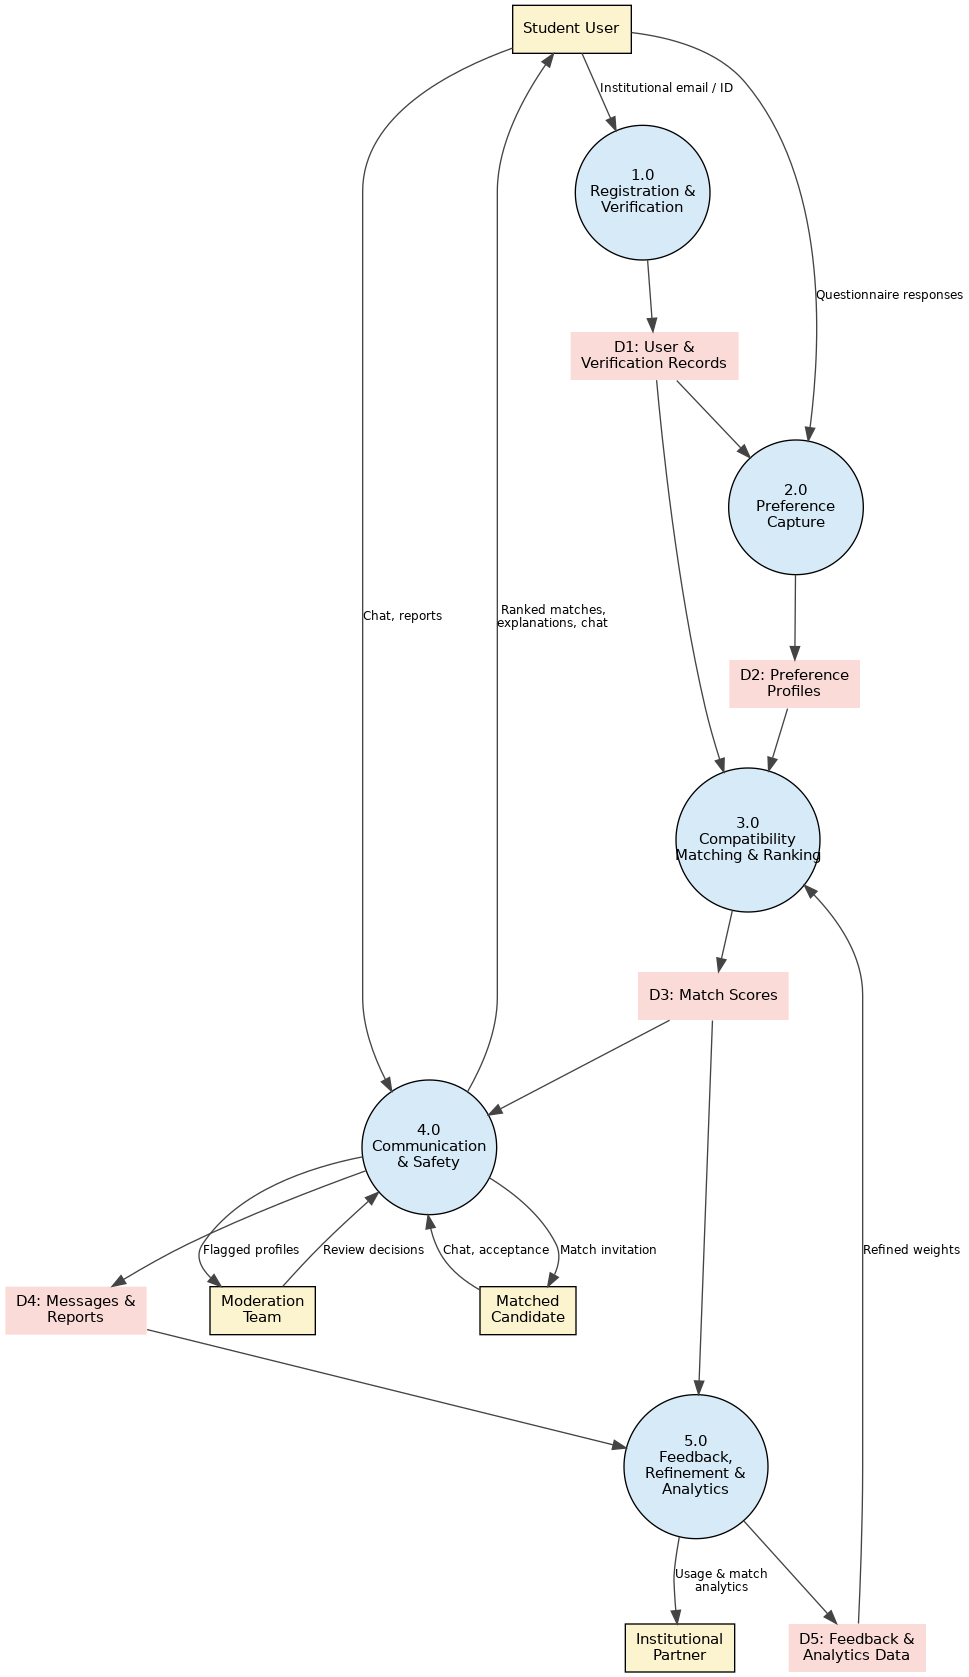
\includegraphics[height=0.82\textheight]{images/image5.png}
    \caption{DFD Level 1 -- Major Process Decomposition}
    \label{fig:4.2}
\end{figure}

The Level-1 DFD shown in Figure \ref{fig:4.2} decomposes the roommate-matching system into five major processes. A student's institutional email/ID first passes through Registration \& Verification (1.0), producing a verified record in D1. Preference Capture (2.0) stores structured questionnaire responses in D2. Compatibility Matching \& Ranking (3.0) reads both D1 and D2 for the eligible candidate pool, computes similarity scores, and writes them to D3. Communication \& Safety (4.0) uses D3 to drive match display and in-app chat, logging messages and reports in D4, and exchanging review decisions with the moderation team. Feedback, Refinement \& Analytics (5.0) aggregates D3 and D4 into D5, feeding refined weights back into process 3.0 and usage analytics out to institutional partners.

% ==================================================================
\chapter{Use Case Diagram}

\begin{itemize}[noitemsep]
    \item \textbf{Student User} -- registers and verifies a profile, completes the preference questionnaire, reviews ranked matches and their explanations, starts in-app chat, reports profiles, and submits match-outcome feedback.
\vspace{2mm}
    \item \textbf{Matched Roommate Candidate} -- registers/verifies, receives match invitations, chats with the seeker, and submits feedback.
\vspace{2mm}
    \item \textbf{Moderator / Safety Team} -- reviews flagged reports and suspends or actions accounts.
\vspace{2mm}
    \item \textbf{Institutional Partner Admin} -- views the institutional analytics dashboard.
\end{itemize}

\begin{figure}[htbp]
    \centering
    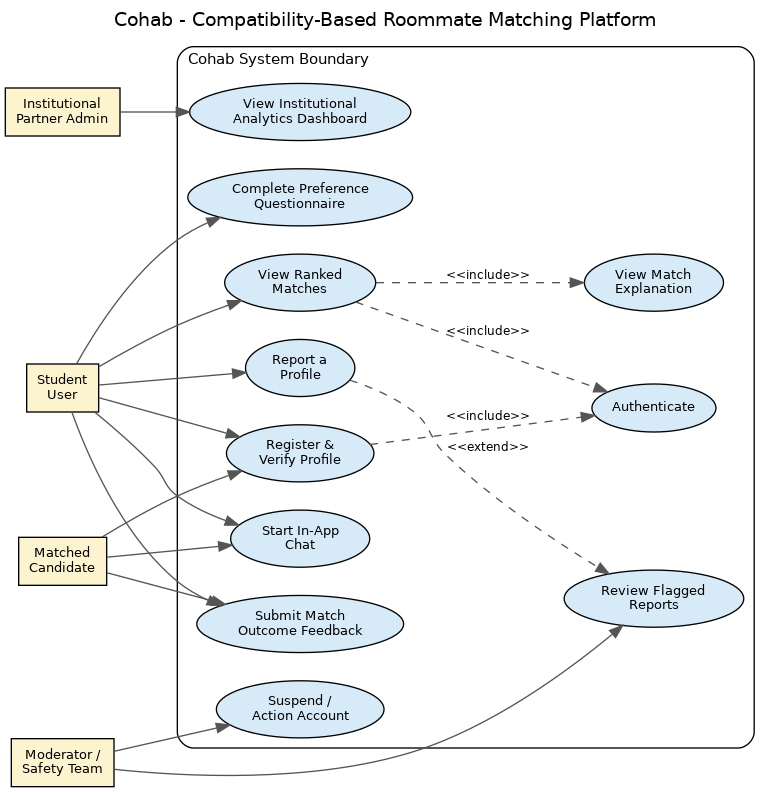
\includegraphics[width=1.0\textwidth]{images/image6.png}
    \caption{Use Case Diagram -- Cohab}
    \label{fig:5.1}
\end{figure}

Figure \ref{fig:5.1} illustrates the interactions between external actors and the Cohab platform. Student users initiate the workflow by registering and verifying their profile, completing the preference questionnaire, and reviewing AI-ranked, explainable matches. Registering a profile and viewing ranked matches both include the Authenticate use case, and viewing ranked matches includes viewing the underlying match explanation. Students and matched candidates use in-app chat to communicate before sharing contact details, and either party can report a profile, which extends into the moderator's report-review use case. Institutional partner admins interact with the system only through the analytics dashboard, keeping their access strictly read-only and anonymised.

% ==================================================================
\chapter{Entity Relationship Diagram (ERD)}

\section{ER Diagram}

The Entity Relationship Diagram (ERD) models the database entities involved in profile verification, preference capture, compatibility scoring, in-app communication, safety reporting, and feedback-driven weight refinement. The design follows a normalised relational schema where primary keys (PK) uniquely identify records and foreign keys (FK) maintain relationships between entities.
\vspace{4mm}
\begin{figure}[htbp]
    \centering
    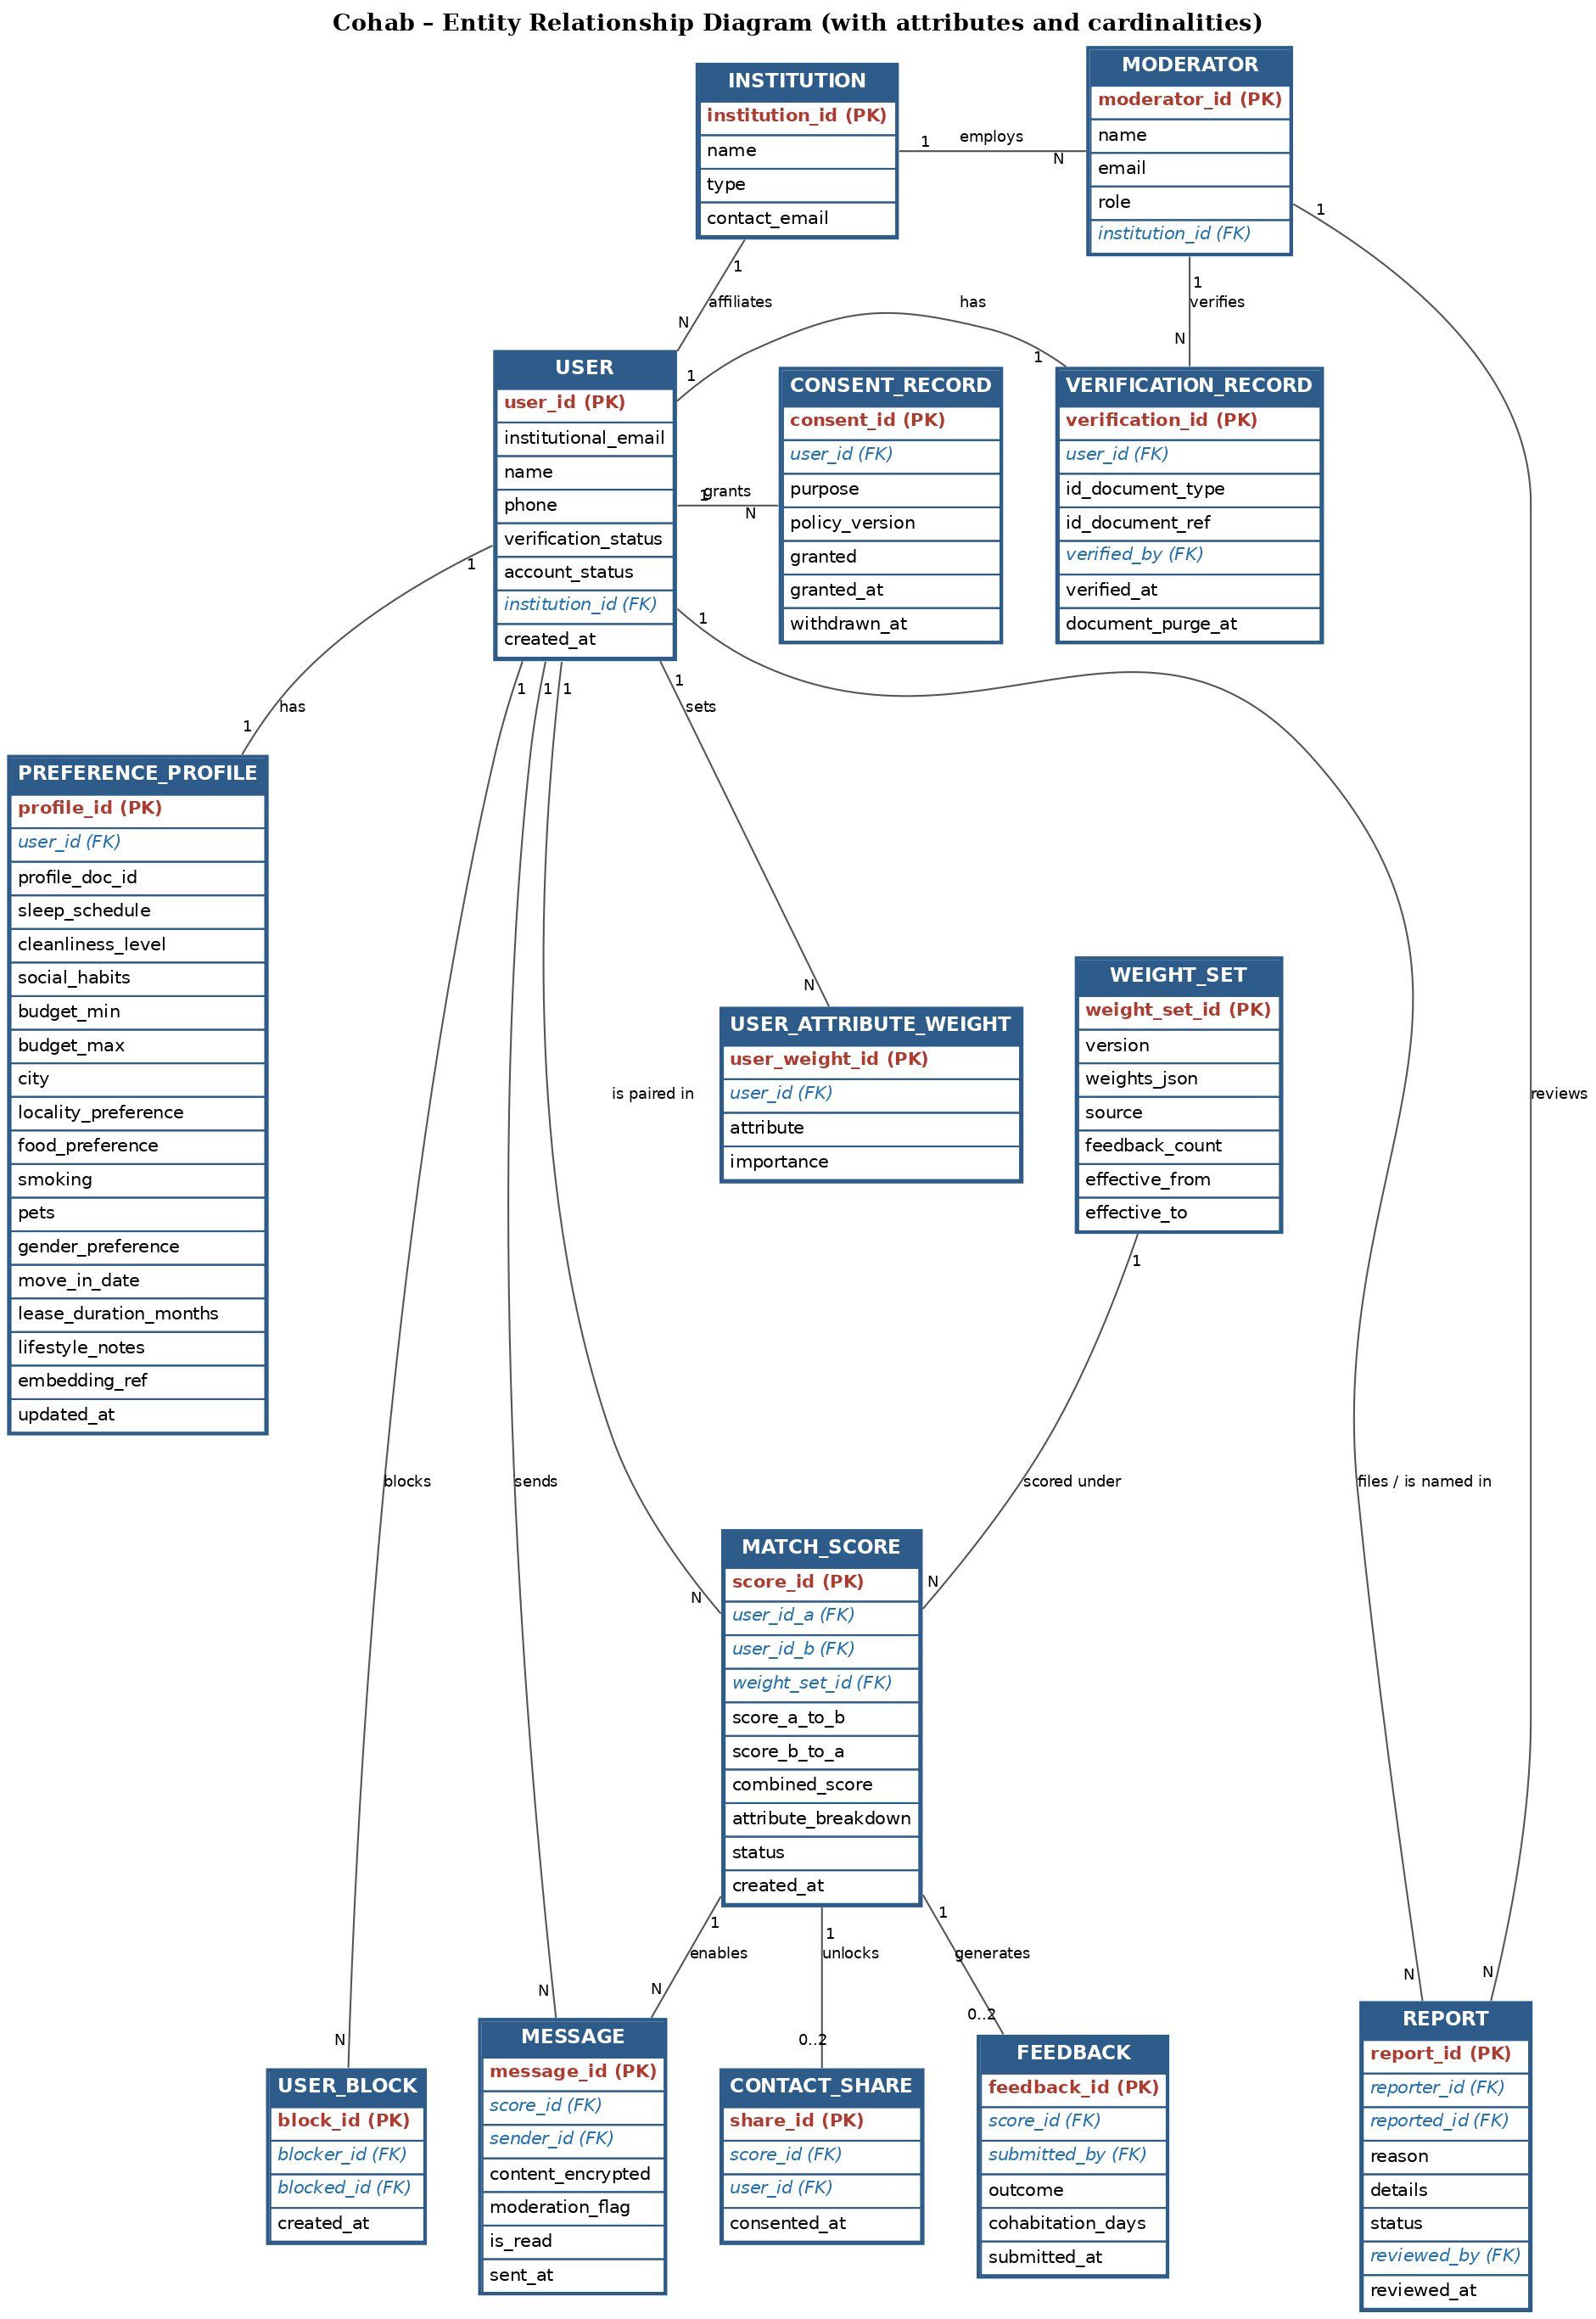
\includegraphics[width=1.0\textwidth]{image7.png}
    \caption{Entity Relationship Diagram}
    \label{fig:6.1}
\end{figure}

The ERD shown in Figure \ref{fig:6.1} models the database structure required to support verification, preference capture, eligibility filtering, compatibility scoring, in-app communication, safety reporting, consent management, and analytics. Candidate information, preference profiles, match scores, messages, and reports are stored in separate tables connected through primary and foreign key relationships, ensuring data integrity and reducing redundancy while supporting future extensions such as group matching.

Six entities have been added relative to the initial draft, each in response to a specific design obligation rather than for completeness. \texttt{MODERATOR} exists because \texttt{REPORT.reviewed\_by} and \texttt{VERIFICATION\_RECORD.verified\_by} identify an accountable person, and an unconstrained free-text field cannot support an audit. \texttt{WEIGHT\_SET} exists because the scoring weights change over time; without recording which weight set produced a given score, an explanation shown to a user in one month cannot be reproduced in the next, which would silently defeat the Explainability requirement. \texttt{USER\_ATTRIBUTE\_WEIGHT} stores each user's own declared importance ratings, which the directional scoring in Section 10.3 requires. \texttt{CONTACT\_SHARE} records the mutual opt-in that the activity diagram already depicts but that the original schema had nowhere to store. \texttt{USER\_BLOCK} supports the block action described in Chapter 11. \texttt{CONSENT\_RECORD} captures purpose-specific consent and its withdrawal, as required under the DPDP Act, 2023.

\subsection*{Cardinality Relationships}

\begin{itemize}[noitemsep]
    \item One INSTITUTION can be affiliated with many USER records, and employs many MODERATOR records (1 : N).
    \item One USER has exactly one VERIFICATION RECORD (1 : 1); one MODERATOR may verify many verification records (1 : N).
    \item One USER has exactly one PREFERENCE PROFILE (1 : 1), whose relational row references an evolving MongoDB document through \texttt{profile\_doc\_id}.
    \item One USER sets many USER ATTRIBUTE WEIGHT records, one per scored attribute (1 : N).
    \item One USER can participate in many MATCH SCORE records as either side of a candidate pair; this many-to-many relationship between users is resolved through the MATCH SCORE table.
    \item One WEIGHT SET governs many MATCH SCORE records (1 : N); every score records the weight set under which it was computed.
    \item One MATCH SCORE, once mutual, enables many MESSAGE records exchanged between the two matched users (1 : N).
    \item One MATCH SCORE can accumulate at most two CONTACT SHARE records --- one consent per participant --- and contact details are released only when both exist (1 : 0..2).
    \item One MATCH SCORE can generate at most two FEEDBACK records, since each participant reports their own outcome independently (1 : 0..2).
    \item One USER can file, or be named in, many REPORT records, and can block many other users (1 : N).
    \item One MODERATOR reviews many REPORT records (1 : N).
\end{itemize}

\subsection*{Integrity Constraints}

The following constraints are part of the schema design rather than application-level conventions, because each of them prevents a class of defect that is difficult to detect after the fact.

\begin{itemize}[noitemsep]
    \item \texttt{MATCH\_SCORE}: \texttt{CHECK (user\_id\_a < user\_id\_b)} together with \texttt{UNIQUE (user\_id\_a, user\_id\_b)}. A user pair is unordered, so without canonicalising the ordering the same pair could be inserted twice as $(a,b)$ and $(b,a)$, producing duplicate match cards and double-counting every downstream analytics figure.
    \item \texttt{FEEDBACK}: \texttt{UNIQUE (score\_id, submitted\_by)}. Each participant may submit exactly one outcome per match; the pair, not \texttt{score\_id} alone, is the natural key.
    \item \texttt{CONTACT\_SHARE}: \texttt{UNIQUE (score\_id, user\_id)}, ensuring consent is recorded once per participant and that the ``both parties opted in'' test is a simple count of two.
    \item \texttt{USER\_BLOCK}: \texttt{UNIQUE (blocker\_id, blocked\_id)} and \texttt{CHECK (blocker\_id <> blocked\_id)}.
    \item \texttt{PREFERENCE\_PROFILE}: \texttt{CHECK (budget\_min <= budget\_max)}.
    \item Supporting indexes: a composite index on \texttt{(city, budget\_min, budget\_max, move\_in\_date)} to serve the Stage-1 eligibility filter described in Section 10.2, and an index on \texttt{MATCH\_SCORE(user\_id\_a, combined\_score DESC)} to serve ranked retrieval without a sort at query time.
\end{itemize}

\section{Data Dictionary}

\subsection*{USER}
\begin{longtable}{L{3.2cm}L{2.5cm}L{8.5cm}}
\toprule
\textbf{Field} & \textbf{Type} & \textbf{Description} \\
\midrule
\endhead
user\_id (PK) & INT &  Unique identifier for a registered user \\
institutional\_email & VARCHAR(100) &  Verified institutional email or government ID reference \\
name & VARCHAR(100) &  User's full name \\
phone & VARCHAR(15) &  Contact number (withheld from other users until both opt in) \\
verification\_status & VARCHAR(20) &  Pending, Verified, or Rejected \\
account\_status & VARCHAR(20) &  Active, Suspended, Banned, or Erased \\
institution\_id (FK) & INT &  Foreign key referencing INSTITUTION(institution\_id) \\
created\_at & DATETIME &  Account creation timestamp \\
\bottomrule
\end{longtable}

\subsection*{MODERATOR}
\begin{longtable}{L{3.2cm}L{2.5cm}L{8.5cm}}
\toprule
\textbf{Field} & \textbf{Type} & \textbf{Description} \\
\midrule
\endhead
moderator\_id (PK) & INT & Unique moderator identifier \\
name & VARCHAR(100) & Moderator's full name \\
email & VARCHAR(100) & Work email address \\
role & VARCHAR(20) & Reviewer, Senior Reviewer, or Administrator \\
institution\_id (FK) & INT & Institution the moderator acts for; NULL for platform staff \\
\bottomrule
\end{longtable}

\subsection*{VERIFICATION RECORD}
\begin{longtable}{L{3.2cm}L{2.5cm}L{8.5cm}}
\toprule
\textbf{Field} & \textbf{Type} & \textbf{Description} \\
\midrule
\endhead
verification\_id (PK) & INT & Unique verification record identifier \\
user\_id (FK) & INT & Foreign key referencing USER(user\_id) \\
id\_document\_type & VARCHAR(30) & Institutional email, student ID, or government ID \\
id\_document\_ref & VARCHAR(200) & Object-store key for the uploaded document; never exposed through any user-facing endpoint \\
verified\_by (FK) & INT & Foreign key referencing MODERATOR(moderator\_id); NULL when verification was automated \\
verified\_at & DATETIME & Timestamp of successful verification \\
document\_purge\_at & DATETIME & Scheduled deletion date for the stored document (verification date + 90 days) \\
\bottomrule
\end{longtable}

\subsection*{CONSENT\_RECORD}
\begin{longtable}{L{3.2cm}L{2.5cm}L{8.5cm}}
\toprule
\textbf{Field} & \textbf{Type} & \textbf{Description} \\
\midrule
\endhead
consent\_id (PK) & INT & Unique consent record identifier \\
user\_id (FK) & INT & Foreign key referencing USER(user\_id) \\
purpose & VARCHAR(40) & Matching, Communication, Analytics, or Marketing --- consent is recorded per purpose, not once globally \\
policy\_version & VARCHAR(20) & Version of the privacy notice the user agreed to \\
granted & BOOLEAN & Whether consent is currently in force \\
granted\_at & DATETIME & Timestamp consent was given \\
withdrawn\_at & DATETIME & Timestamp consent was withdrawn; NULL while active \\
\bottomrule
\end{longtable}

\subsection*{PREFERENCE PROFILE}
\begin{longtable}{L{3.2cm}L{2.5cm}L{8.5cm}}
\toprule
\textbf{Field} & \textbf{Type} & \textbf{Description} \\
\midrule
\endhead
profile\_id (PK) & INT & Unique preference profile identifier \\
user\_id (FK) & INT & Foreign key referencing USER(user\_id) \\
profile\_doc\_id & VARCHAR(40) & Reference to the full questionnaire document in MongoDB \\
sleep\_schedule & VARCHAR(20) & Early riser, night owl, flexible, etc. \\
cleanliness\_level & VARCHAR(20) & Self-reported cleanliness expectation \\
social\_habits & VARCHAR(20) & Guest frequency and socialising preference \\
budget\_min & INT & Lower bound of monthly budget, in rupees \\
budget\_max & INT & Upper bound of monthly budget, in rupees \\
city & VARCHAR(50) & City of intended residence; a Stage-1 hard constraint \\
locality\_preference & VARCHAR(100) & Preferred campus / neighbourhood within the city \\
food\_preference & VARCHAR(20) & Dietary preference (veg / non-veg / vegan, etc.) \\
smoking & VARCHAR(20) & Own habit and tolerance of a smoking roommate \\
pets & VARCHAR(20) & Own pets and tolerance of a roommate's pets \\
gender\_preference & VARCHAR(20) & Declared roommate gender preference; evaluated mutually as a hard constraint \\
move\_in\_date & DATE & Intended move-in date \\
lease\_duration\_months & INT & Intended length of stay \\
lifestyle\_notes & TEXT & Free-text description used for semantic similarity \\
embedding\_ref & VARCHAR(60) & Cache key for the precomputed sentence-transformer embedding of \texttt{lifestyle\_notes} \\
updated\_at & DATETIME & Timestamp of the last questionnaire edit; invalidates cached scores \\
\bottomrule
\end{longtable}

\vspace{2mm}
\noindent\textit{Note.} \texttt{budget\_min} and \texttt{budget\_max} replace the earlier single \texttt{budget\_range VARCHAR(30)} field. The scoring algorithm in Section 10.3 computes a normalised absolute difference over budget, which is not defined on a string; storing the bounds as integers also allows the Stage-1 filter to test band intersection directly in SQL.

\subsection*{USER\_ATTRIBUTE\_WEIGHT}
\begin{longtable}{L{3.2cm}L{2.5cm}L{8.5cm}}
\toprule
\textbf{Field} & \textbf{Type} & \textbf{Description} \\
\midrule
\endhead
user\_weight\_id (PK) & INT & Unique identifier \\
user\_id (FK) & INT & Foreign key referencing USER(user\_id) \\
attribute & VARCHAR(30) & Scored attribute the rating applies to \\
importance & FLOAT & User's declared importance for that attribute, normalised to sum to 1 across the user's rows \\
\bottomrule
\end{longtable}

\subsection*{WEIGHT\_SET}
\begin{longtable}{L{3.2cm}L{2.5cm}L{8.5cm}}
\toprule
\textbf{Field} & \textbf{Type} & \textbf{Description} \\
\midrule
\endhead
weight\_set\_id (PK) & INT & Unique weight set identifier \\
version & INT & Monotonically increasing version number \\
weights\_json & TEXT (JSON) & Platform-level default weight vector, summing to 1 \\
source & VARCHAR(20) & Expert (initial, hand-assigned) or Learned (derived from outcome data) \\
feedback\_count & INT & Number of outcome records the weight set was derived from \\
effective\_from & DATETIME & Start of the period during which this set was active \\
effective\_to & DATETIME & End of that period; NULL for the currently active set \\
\bottomrule
\end{longtable}

\subsection*{MATCH SCORE}
\begin{longtable}{L{3.2cm}L{2.5cm}L{8.5cm}}
\toprule
\textbf{Field} & \textbf{Type} & \textbf{Description} \\
\midrule
\endhead
score\_id (PK) & INT & Unique match-score record identifier \\
user\_id\_a (FK) & INT & Foreign key referencing USER(user\_id); by constraint the lower of the two identifiers \\
user\_id\_b (FK) & INT & Foreign key referencing USER(user\_id); the higher of the two identifiers \\
weight\_set\_id (FK) & INT & Foreign key referencing WEIGHT\_SET(weight\_set\_id) --- the weights this score was computed under \\
score\_a\_to\_b & FLOAT & How well B satisfies A's stated priorities, 0--1 \\
score\_b\_to\_a & FLOAT & How well A satisfies B's stated priorities, 0--1 \\
combined\_score & FLOAT & Harmonic mean of the two directional scores, 0--1 \\
attribute\_breakdown & TEXT (JSON) & Per-attribute similarity values used for explainability \\
status & VARCHAR(20) & Suggested, Viewed, Interested, Mutual, Chatting, Contact Shared, Cohabiting, Rejected, or Expired (see Figure \ref{fig:8.2}) \\
created\_at & DATETIME & Timestamp the score was computed \\
\bottomrule
\end{longtable}

\subsection*{MESSAGE}
\begin{longtable}{L{3.2cm}L{2.5cm}L{8.5cm}}
\toprule
\textbf{Field} & \textbf{Type} & \textbf{Description} \\
\midrule
\endhead
message\_id (PK) & INT & Unique message identifier \\
score\_id (FK) & INT & Foreign key referencing MATCH SCORE(score\_id) \\
sender\_id (FK) & INT & Foreign key referencing USER(user\_id) \\
content\_encrypted & TEXT & Message content, encrypted at rest under a server-held key (see Section 11.3) \\
moderation\_flag & VARCHAR(20) & Clean, Auto-Flagged, or Confirmed-Abusive \\
is\_read & BOOLEAN & Whether the recipient has opened the message \\
sent\_at & DATETIME & Timestamp the message was sent \\
\bottomrule
\end{longtable}

\subsection*{CONTACT\_SHARE}
\begin{longtable}{L{3.2cm}L{2.5cm}L{8.5cm}}
\toprule
\textbf{Field} & \textbf{Type} & \textbf{Description} \\
\midrule
\endhead
share\_id (PK) & INT & Unique consent record identifier \\
score\_id (FK) & INT & Foreign key referencing MATCH SCORE(score\_id) \\
user\_id (FK) & INT & The participant granting consent to release their contact details \\
consented\_at & DATETIME & Timestamp of the opt-in \\
\bottomrule
\end{longtable}

\subsection*{USER\_BLOCK}
\begin{longtable}{L{3.2cm}L{2.5cm}L{8.5cm}}
\toprule
\textbf{Field} & \textbf{Type} & \textbf{Description} \\
\midrule
\endhead
block\_id (PK) & INT & Unique block record identifier \\
blocker\_id (FK) & INT & User who initiated the block \\
blocked\_id (FK) & INT & User who was blocked \\
created\_at & DATETIME & Timestamp the block was applied \\
\bottomrule
\end{longtable}

\subsection*{REPORT}
\begin{longtable}{L{3.2cm}L{2.5cm}L{8.5cm}}
\toprule
\textbf{Field} & \textbf{Type} & \textbf{Description} \\
\midrule
\endhead
report\_id (PK) & INT & Unique report identifier \\
reporter\_id (FK) & INT & Foreign key referencing USER(user\_id) --- user filing the report \\
reported\_id (FK) & INT & Foreign key referencing USER(user\_id) --- user being reported \\
reason & VARCHAR(50) & Suspicious, abusive, or misrepresented profile, etc. \\
details & TEXT & Additional context supplied by the reporter \\
status & VARCHAR(20) & Open, Under Review, Substantiated, Dismissed, or Action Taken (see Figure \ref{fig:8.2}) \\
reviewed\_by (FK) & INT & Foreign key referencing MODERATOR(moderator\_id) \\
reviewed\_at & DATETIME & Timestamp of moderation decision \\
\bottomrule
\end{longtable}

\subsection*{FEEDBACK}
\begin{longtable}{L{3.2cm}L{2.5cm}L{8.5cm}}
\toprule
\textbf{Field} & \textbf{Type} & \textbf{Description} \\
\midrule
\endhead
feedback\_id (PK) & INT & Unique feedback record identifier \\
score\_id (FK) & INT & Foreign key referencing MATCH SCORE(score\_id) \\
outcome & VARCHAR(20) & Pursued, Accepted, Conflict, or Rejected \\
cohabitation\_days & INT & Days the pair actually lived together at the time of reporting; NULL if they never moved in. This is the closest available proxy for whether the match succeeded \\
submitted\_by (FK) & INT & Foreign key referencing USER(user\_id) \\
submitted\_at & DATETIME & Timestamp the feedback was submitted \\
\bottomrule
\end{longtable}

\subsection*{INSTITUTION}
\begin{longtable}{L{3.2cm}L{2.5cm}L{8.5cm}}
\toprule
\textbf{Field} & \textbf{Type} & \textbf{Description} \\
\midrule
\endhead
institution\_id (PK) & INT & Unique institution / operator identifier \\
name & VARCHAR(100) & Campus or PG/co-living operator name \\
type & VARCHAR(20) & Campus or PG Operator \\
contact\_email & VARCHAR(100) & Primary contact email for the partner administrator \\
\bottomrule
\end{longtable}

% ==================================================================
\chapter{Class Diagram}

\section{Design Rationale}

Per the Reusability non-functional requirement in the SRS, business-logic modules (authentication, preference, matcher, ranker, chat, safety reporting, feedback, analytics) are implemented as independent Python classes with well-defined interfaces, allowing new modules such as group/multi-person matching or campus room-allocation integration, per the Future Scope to be added without modifying existing code.

\begin{figure}[htbp]
    \centering
    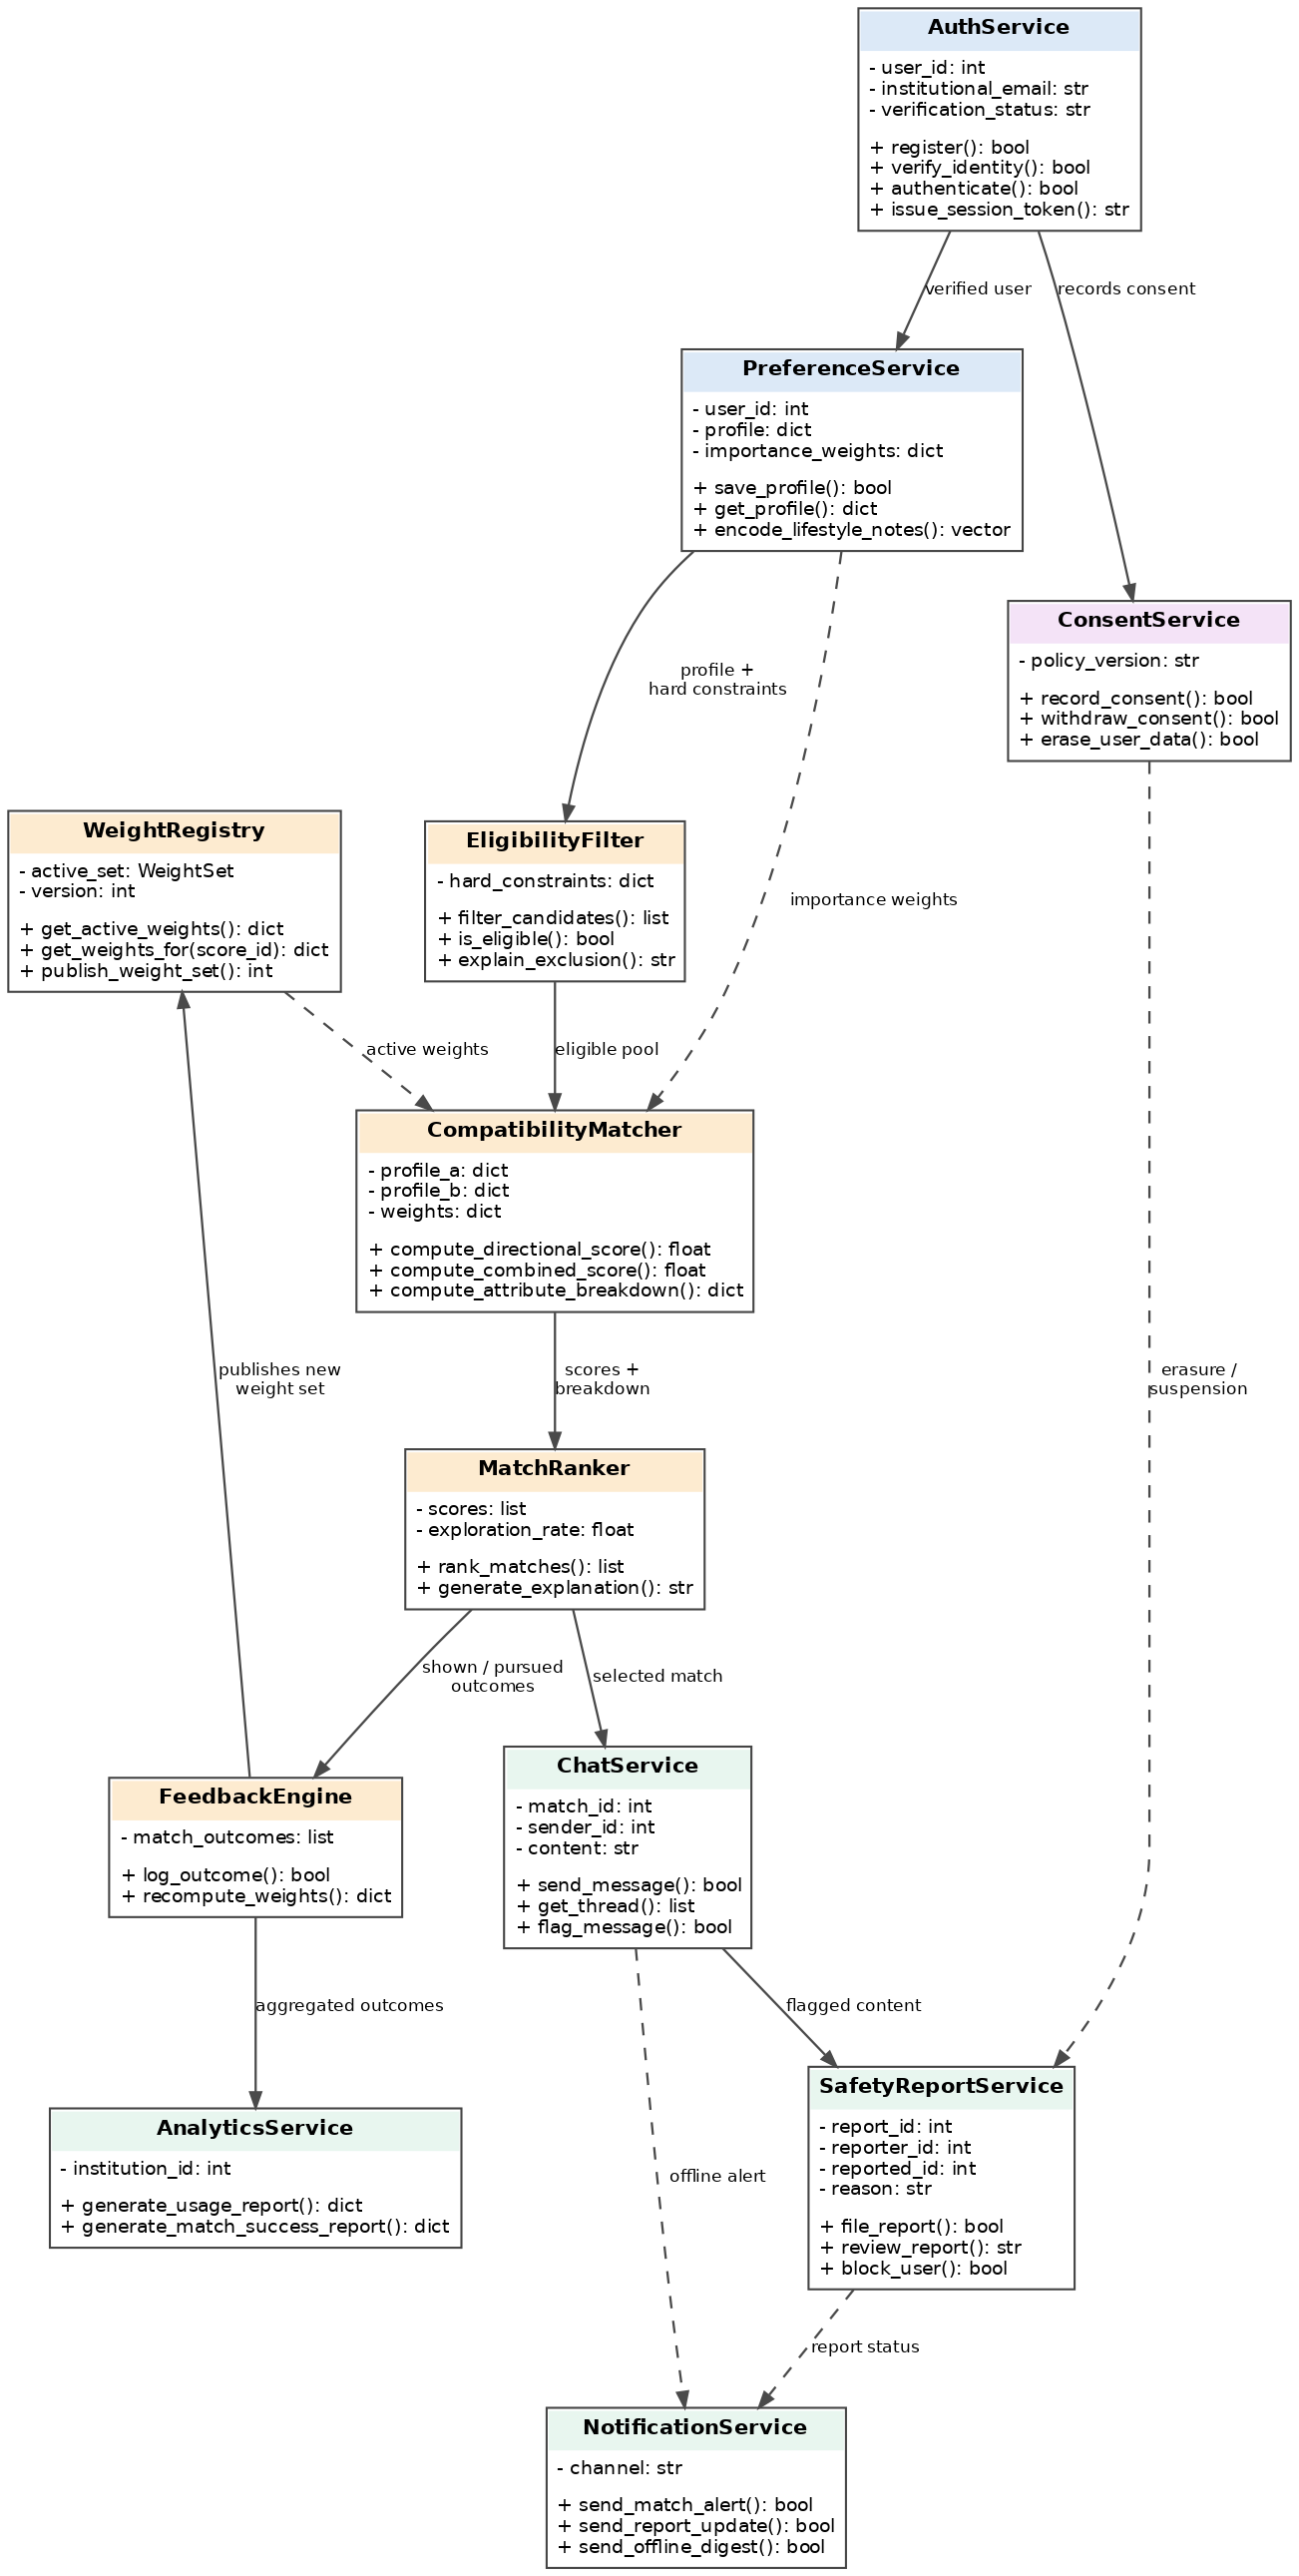
\includegraphics[height=0.78\textheight]{images/image8.png}
    \caption{Class Diagram -- Core Business Logic Modules}
    \label{fig:7.1}
\end{figure}

Figure \ref{fig:7.1} presents the object-oriented structure of Cohab. Independent classes are used for authentication, preference management, eligibility filtering, compatibility matching, ranking, chat, safety reporting, notification, consent handling, and feedback-driven weight refinement to ensure modularity and maintainability.

\texttt{AuthService} validates institutional identity and issues session tokens; \texttt{PreferenceService} stores and retrieves the structured questionnaire responses, the user's declared importance weights, and the precomputed embedding of their lifestyle notes; \texttt{EligibilityFilter} reduces the candidate pool to those who satisfy every hard constraint, and retains the reason for each exclusion; \texttt{WeightRegistry} owns the versioned platform weight vectors and answers both ``what weights are active now'' and ``what weights produced this historical score''; \texttt{CompatibilityMatcher} computes the two directional scores, their harmonic mean, and the per-attribute breakdown for a pair of profiles; \texttt{MatchRanker} sorts scored candidates and generates the plain-language explanation shown to the user; \texttt{ChatService} manages the moderated in-app conversation thread for a mutual match; \texttt{SafetyReportService} files and reviews reports and applies blocks; \texttt{NotificationService} centralises email and SMS delivery so that no business class talks to a transport directly; \texttt{ConsentService} records purpose-specific consent and executes erasure requests; \texttt{FeedbackEngine} logs match outcomes and periodically recomputes attribute weights; and \texttt{AnalyticsService} produces the aggregated institutional reports.

Two aspects of the dependency structure are deliberate. First, the classes do not form a single linear chain: \texttt{EligibilityFilter} and \texttt{WeightRegistry} both feed \texttt{CompatibilityMatcher} independently, and the safety, notification and consent classes sit on separate paths, which is what makes them independently replaceable in the sense the Reusability requirement intends. Second, the refinement loop is closed through \texttt{WeightRegistry} rather than by having \texttt{FeedbackEngine} write directly into \texttt{CompatibilityMatcher}. A direct write would create a cycle between the two classes and, more importantly, would leave no record of which weight vector produced a given historical score. Publishing a new versioned weight set instead keeps the dependency graph acyclic and preserves reproducibility of explanations. This separation enables the future extensions described in Chapter 10 --- the learned ranking function and the stable-matching batch mode --- without significant changes to the existing codebase.

\vspace{4mm}

\section{Object Diagram}

While the class diagram in Figure \ref{fig:7.1} shows the static structure of the system, the object diagram below shows a concrete instance snapshot at run time: two verified users, their preference profiles, the CompatibilityMatcher instance comparing them, and the resulting MatchScore object.

\begin{figure}[htbp]
    \centering
    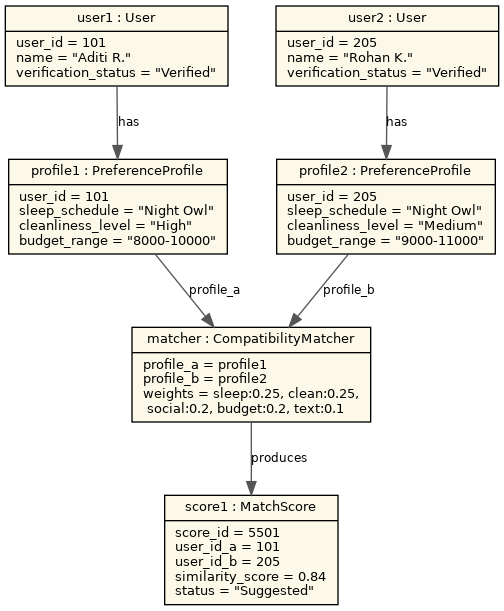
\includegraphics[height=0.68\textheight]{images/image9.png}
    \caption{Object Diagram -- Sample Match Instance}
    \label{fig:7.2}
\end{figure}

Figure \ref{fig:7.2} illustrates a single worked example: user1 (Aditi R.) and user2 (Rohan K.) each have an associated PreferenceProfile object. The matcher object references both profiles and the currently active attribute weights, and produces score1, a MatchScore instance recording a similarity score of 0.84 with status ``Suggested'' --- the same object structure that would be persisted to the MATCH SCORE table described in Section 6.2 and surfaced to the user via the Ranking \& Explainability service.

% ==================================================================
\chapter{Activity Diagram}

\section{Roommate Matching Workflow Activity Diagram}

The activity diagram illustrates the overall workflow of Cohab from sign-up and verification to compatibility scoring, match review, in-app chat, and feedback-driven weight refinement. The diagram highlights the decision points where a user chooses whether to pursue a suggested match, and where both matched users must confirm interest before contact details are exchanged.


\begin{figure}[htbp]
    \centering
    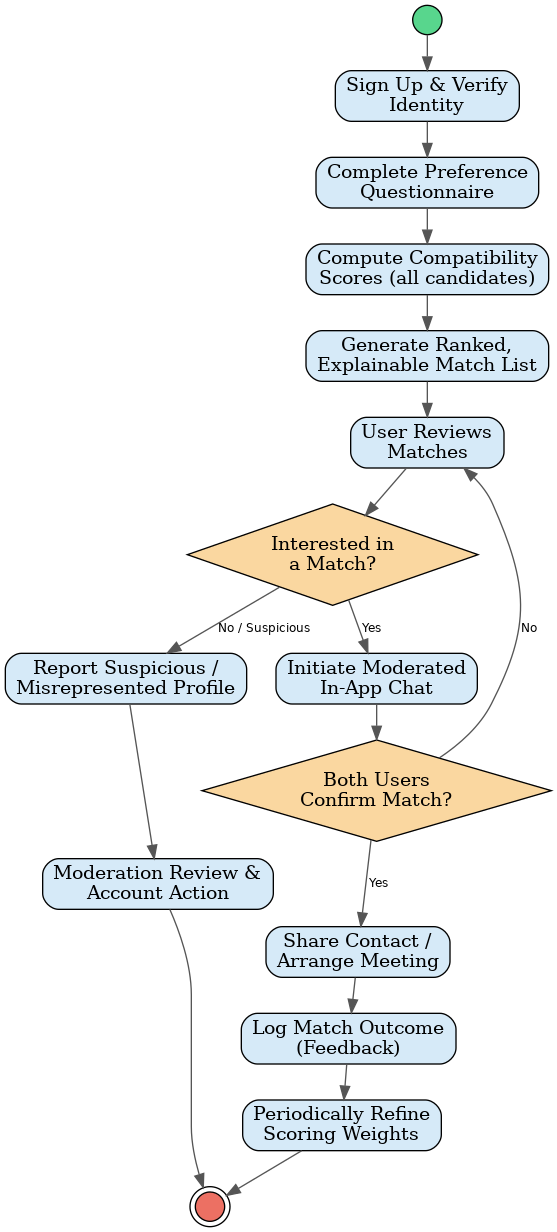
\includegraphics[height=0.78\textheight]{images/image10.png}
    \caption{Activity Diagram -- Roommate Matching Workflow}
    \label{fig:8.1}
\end{figure}

\vspace{4mm}
The workflow begins with sign-up and identity verification, followed by completion of the preference questionnaire. The system computes compatibility scores against all eligible candidates and generates a ranked, explainable match list. If the user is not interested in any suggested match, or flags a profile as suspicious or misrepresented, the profile is routed to the moderation team for review and possible account action. If the user is interested, a moderated in-app chat is initiated; once both users confirm the match, contact details may be shared and the outcome is logged as feedback, which periodically feeds back into recalculating the scoring weights described in Chapter 10.

\section{Match and Report State Models}

The activity diagram captures the intended path through the system, but it does not define the permitted states of the two entities whose status fields drive most of the application's behaviour. Figure \ref{fig:8.2} specifies those state machines explicitly, so that the \texttt{status} columns of \texttt{MATCH\_SCORE} and \texttt{REPORT} have an enumerated domain and a defined set of legal transitions rather than an open set of strings.

\begin{figure}[htbp]
    \centering
    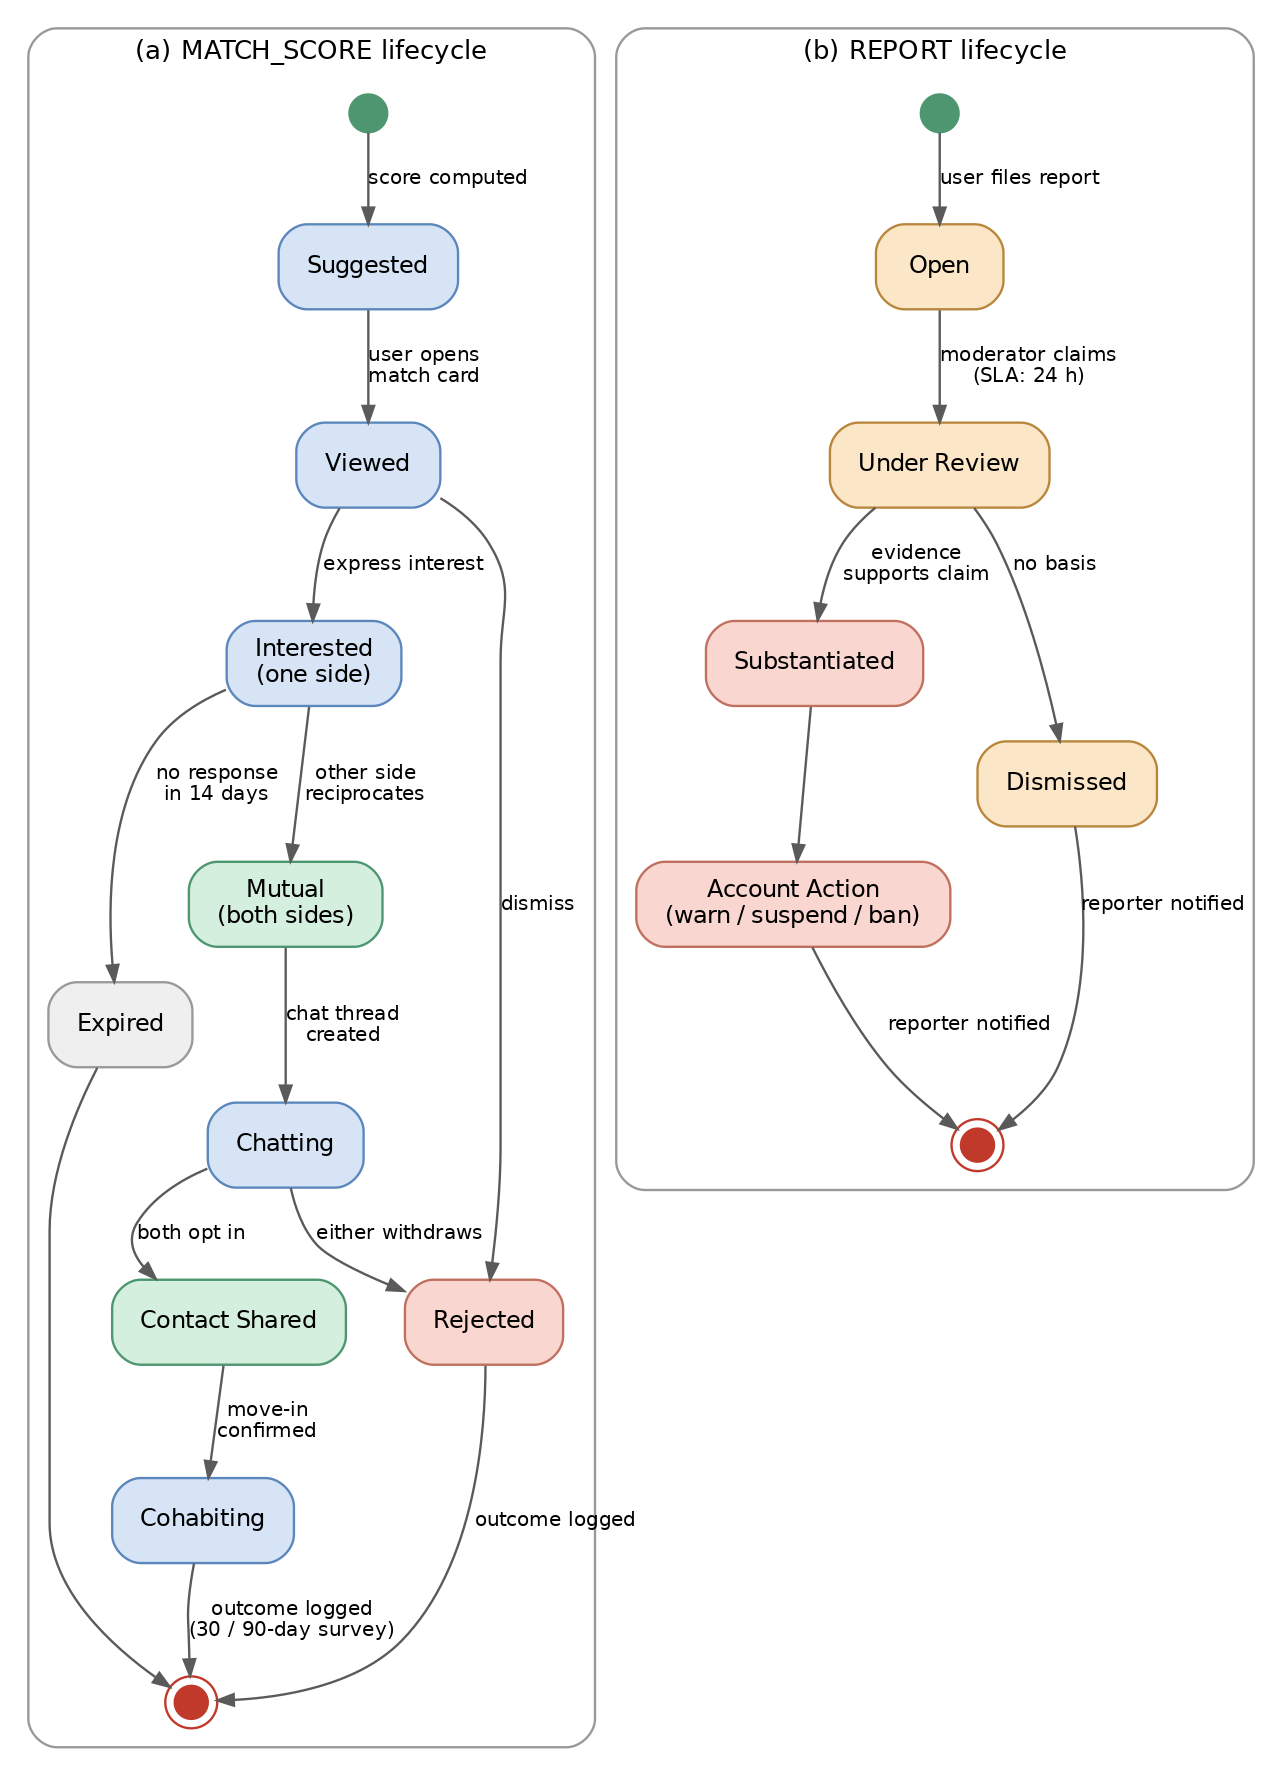
\includegraphics[height=0.74\textheight]{images/image18.png}
    \caption{State Diagrams -- Match Lifecycle and Report Lifecycle}
    \label{fig:8.2}
\end{figure}

Three transitions in Figure \ref{fig:8.2}(a) carry design weight. \emph{Interested} advances to \emph{Mutual} only when the second party reciprocates, which is the mechanism by which the system honours the design objective that no roommate is ever assigned without mutual consent. \emph{Chatting} advances to \emph{Contact Shared} only when two \texttt{CONTACT\_SHARE} rows exist for the match, so contact details cannot be released by a single party's action. The \emph{Expired} state exists because a match left unanswered is neither accepted nor rejected; without it, stale suggestions would accumulate in the candidate's list and would pollute the outcome data used for weight refinement with cases that were never genuinely evaluated.

Figure \ref{fig:8.2}(b) gives the report lifecycle a review service level and separates the finding (\emph{Substantiated} or \emph{Dismissed}) from the sanction (\emph{Account Action}). Keeping the two distinct means the moderation record shows what was concluded as well as what was done, which is what makes the audit trail meaningful when an account action is later challenged.

% ==================================================================
\chapter{Sequence Diagram}

\section{Compatibility Matching and Match List Generation Sequence}

The sequence below illustrates the primary interaction flow when a student submits the preference questionnaire and the system returns a ranked, explainable match list, followed by the initiation of an in-app chat with a selected match.

\vspace{4mm}
\begin{figure}[htbp]
    \centering
    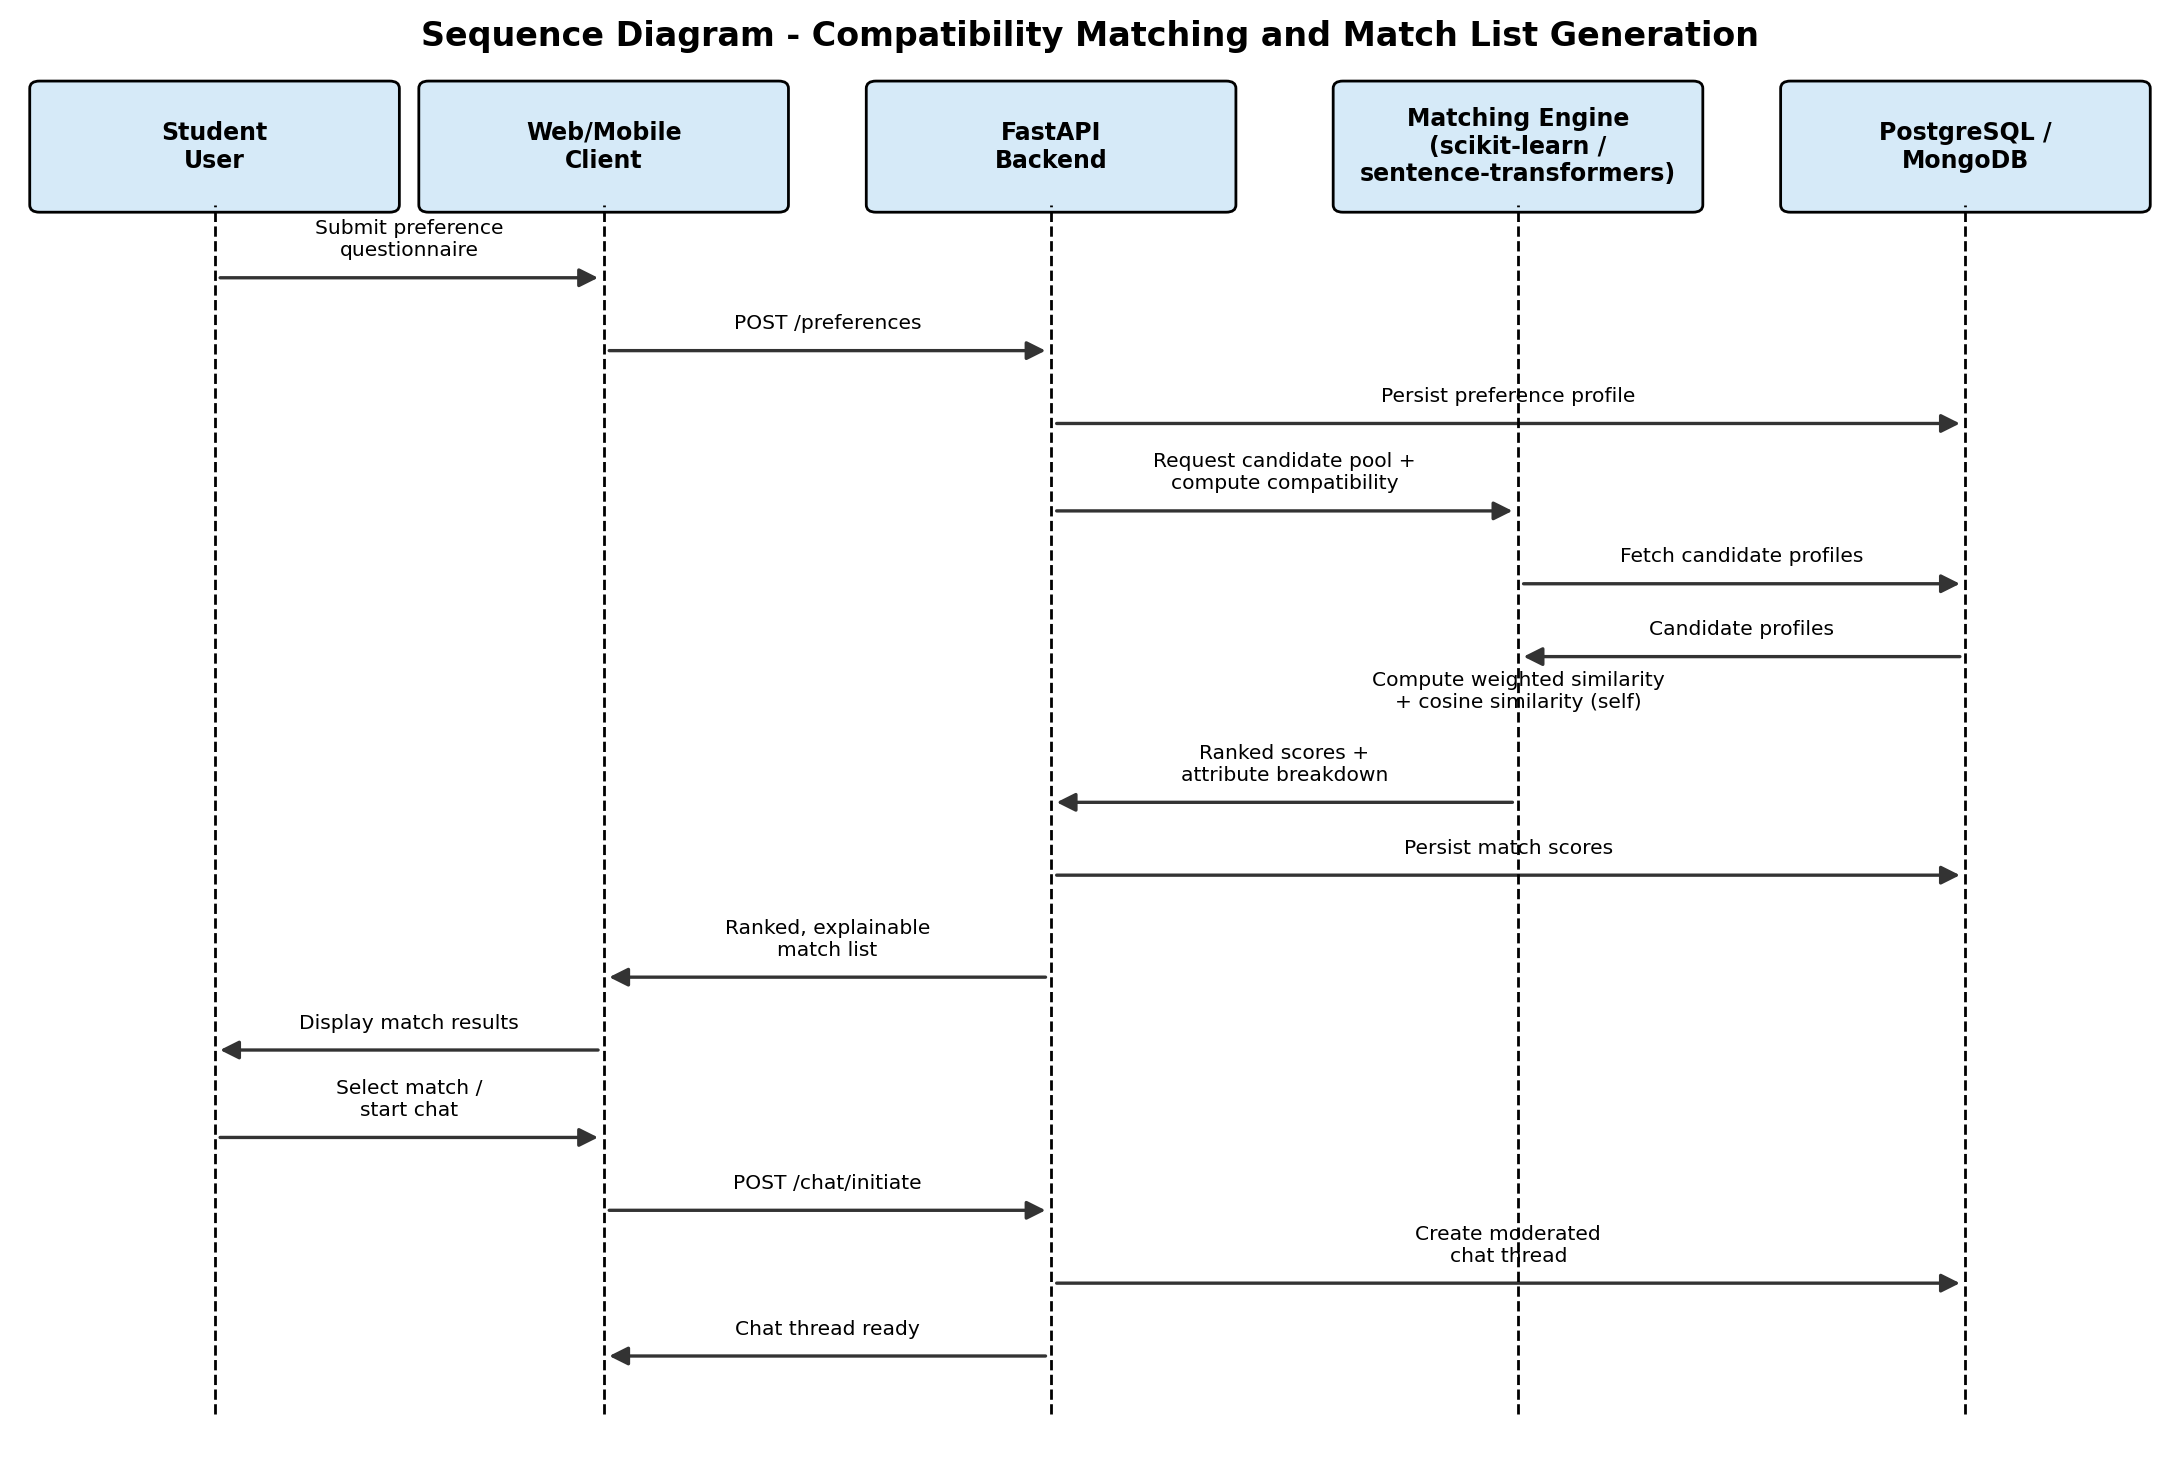
\includegraphics[width=1.0\textwidth]{images/image11.png}
    \caption{Sequence Diagram -- Compatibility Matching and Match List Generation}
    \label{fig:9.1}
\end{figure}

\vspace{4mm}
The sequence diagram shown in Figure \ref{fig:9.1} illustrates the chronological interactions among system components during match generation. The workflow begins when a student submits the preference questionnaire; the FastAPI backend persists the profile in MongoDB and requests the eligible candidate pool from PostgreSQL. The Matching Engine (scikit-learn for weighted structured-attribute similarity, sentence-transformers for semantic similarity on free-text fields) computes ranked scores with an attribute-level breakdown, which the backend persists as match scores and returns to the client for display. When the student selects a match to pursue, the client requests chat initiation, and the backend creates a moderated chat thread between the two users.

\vspace{2mm}
\noindent\textbf{Two timing qualifications.} First, the candidate pool requested from PostgreSQL is the \emph{eligible} pool produced by the Stage-1 filter of Section 10.2, not the full user table; the filter runs as an indexed query rather than as an in-memory pass over every user. Second, the sentence-transformer encoding of a user's lifestyle notes is performed once, when the questionnaire is saved, and the resulting vector is cached and referenced by \texttt{embedding\_ref}. Encoding both profiles inside the request path, as a literal reading of the diagram might suggest, would place a transformer forward pass in the critical path for every candidate and would make the five-second performance target in the SRS unattainable. At match time the engine performs only a cached-vector lookup and a cosine product.

% ==================================================================
\chapter{Algorithms and Data Structures}

\section{Design Approach: Constraints Before Preferences}

Roommate compatibility is not a single graded quantity. Some requirements are negotiable and admit degrees --- one user prefers an early riser but can live with a night owl --- while others are binary and non-negotiable: a candidate in a different city, outside the budget band, or available only from a date six months away is not a weak match but an impossible one.

A single weighted sum cannot express this distinction. If every attribute contributes proportionally to one score, a candidate who scores highly on sleep schedule, cleanliness, social habits and lifestyle notes can accumulate a high overall score while failing on city or budget, and will then be presented to the user as a strong recommendation. Increasing the weight on the critical attributes does not solve the problem; it only raises the score a candidate must reach elsewhere to overcome the failure, and the failure remains compensable in principle.

Cohab therefore separates the two kinds of requirement into two stages, shown in Figure \ref{fig:10.1}. Stage 1 applies hard constraints as a boolean filter that a candidate either passes or fails. Stage 2 applies the weighted, explainable scoring only to candidates that survived Stage 1.

\begin{figure}[htbp]
    \centering
    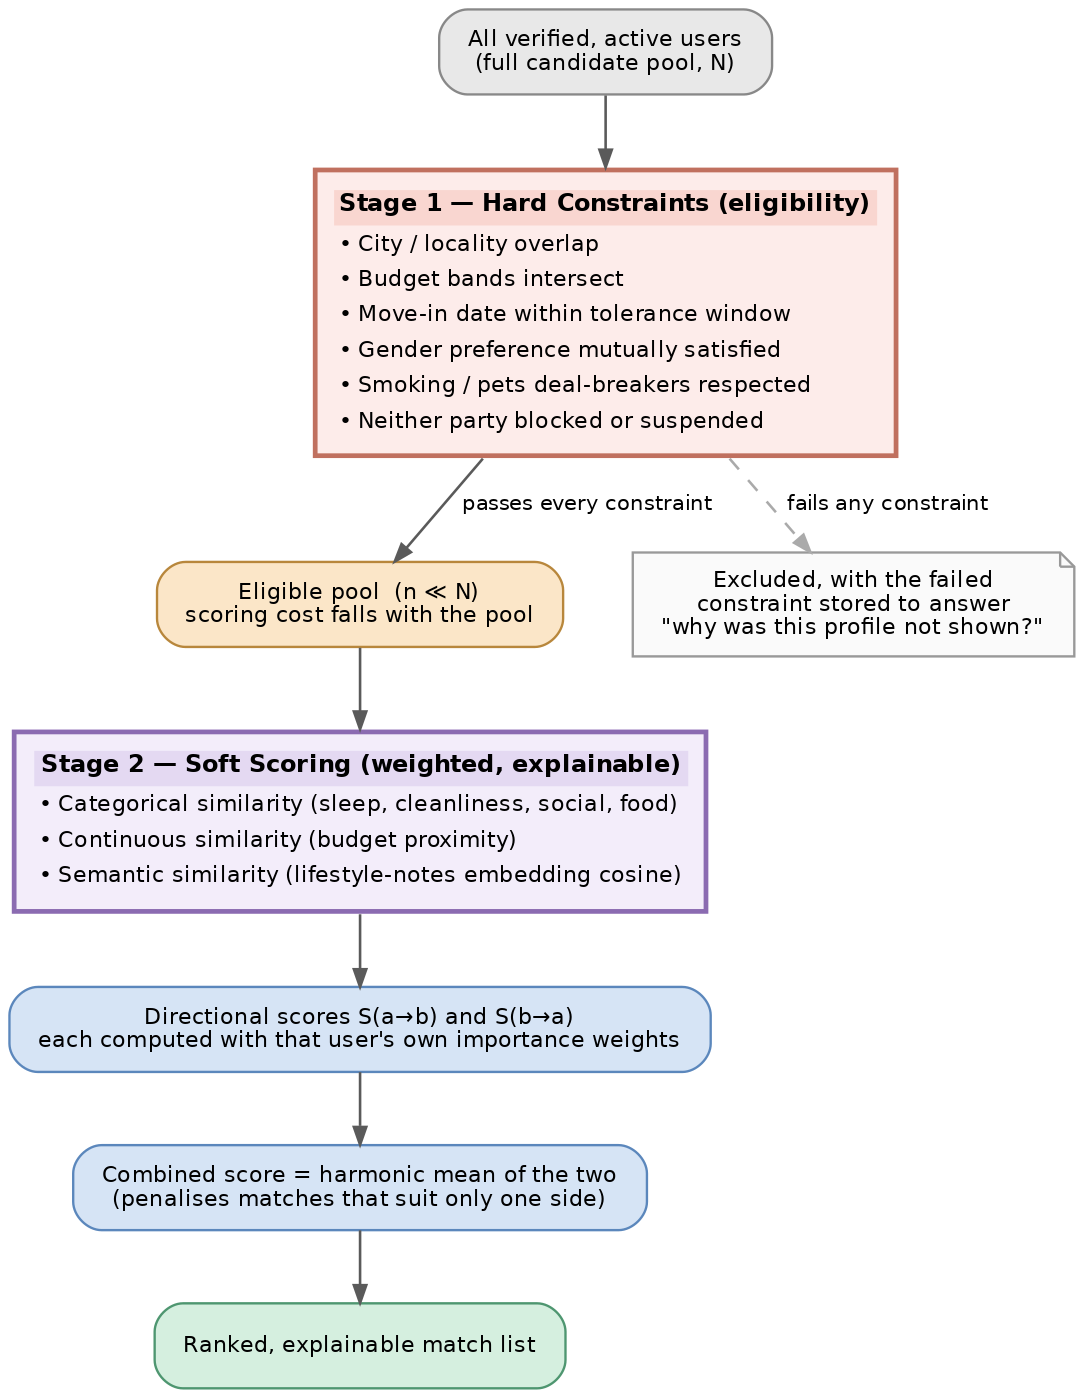
\includegraphics[height=0.72\textheight]{images/image17.png}
    \caption{Two-Stage Matching Pipeline -- Hard Constraints followed by Soft Scoring}
    \label{fig:10.1}
\end{figure}

Besides correctness, the two-stage structure carries a performance consequence. Stage 1 is an indexed relational query, and it typically removes the large majority of the user base before any embedding comparison is attempted. The expensive Stage-2 work is then performed on a pool one or two orders of magnitude smaller, which is what makes the five-second SRS target achievable as the user base grows rather than only at pilot scale.

\section{Stage 1: Eligibility Filtering Algorithm}

\vspace{3mm}
\textbf{Algorithm: FilterEligibleCandidates(user, pool)}
\begin{enumerate}[label=\arabic*., itemsep=0pt]
    \ttfamily
    \item eligible $\leftarrow$ [ ]; excluded $\leftarrow$ \{ \}
    \item for each candidate c in pool:
    \item \quad if c.user\_id = user.user\_id: continue
    \item \quad if c.account\_status $\neq$ Active or c.verification\_status $\neq$ Verified:
    \item \quad\quad excluded[c] $\leftarrow$ "not an active verified account"; continue
    \item \quad if Blocked(user, c) or Blocked(c, user):
    \item \quad\quad excluded[c] $\leftarrow$ "blocked"; continue
    \item \quad if c.city $\neq$ user.city:
    \item \quad\quad excluded[c] $\leftarrow$ "different city"; continue
    \item \quad if c.budget\_max < user.budget\_min or user.budget\_max < c.budget\_min:
    \item \quad\quad excluded[c] $\leftarrow$ "budget bands do not overlap"; continue
    \item \quad if |c.move\_in\_date -- user.move\_in\_date| > TOLERANCE\_DAYS:
    \item \quad\quad excluded[c] $\leftarrow$ "move-in dates too far apart"; continue
    \item \quad if not GenderPreferenceMutuallySatisfied(user, c):
    \item \quad\quad excluded[c] $\leftarrow$ "gender preference not mutual"; continue
    \item \quad if not DealBreakersRespected(user, c):
    \hfill // smoking, pets
    \item \quad\quad excluded[c] $\leftarrow$ "declared deal-breaker"; continue
    \item \quad eligible.append(c)
    \item return eligible, excluded
\end{enumerate}

\vspace{4mm}

Each constraint is evaluated symmetrically: a pair is eligible only if it satisfies both users' requirements, so eligibility is a property of the pair rather than of one user's search. The \texttt{excluded} map is retained rather than discarded, because it allows the interface to answer ``why am I not seeing many matches?'' with a concrete reason, and it gives the pilot a direct measurement of which constraint is most responsible for a thin candidate pool.

\section{Stage 2: Compatibility Scoring Algorithm (MVP)}

The scoring approach combines rule-based weighted similarity across structured questionnaire attributes with cosine similarity on a dense sentence-embedding of each user's free-text lifestyle notes. Categorical attributes use a category-distance function; the continuous budget attribute uses a normalised absolute-difference measure over the midpoints of the two declared budget bands; and the free-text field is compared using sentence-transformer embeddings, so that two loosely-worded but similar lifestyle descriptions still score well.

Scoring is computed \emph{directionally}. Two users rarely care about the same things to the same degree: one may regard budget as decisive and sleep schedule as incidental, while the other takes the opposite view. A single symmetric score with one shared weight vector silently averages these differences away. The algorithm therefore computes $S(a \rightarrow b)$ using A's own importance weights and $S(b \rightarrow a)$ using B's, and combines them with a harmonic mean, which --- unlike an arithmetic mean --- is pulled down sharply when one of the two values is low. A match that suits one party very well and the other poorly is thereby ranked below a match that suits both moderately well, which is the intended behaviour for a shared-living arrangement.

\vspace{4mm}

\textbf{Algorithm: ComputeCompatibilityScore(profile\_a, profile\_b, weight\_set)}
\begin{enumerate}[label=\arabic*., itemsep=0pt]
    \ttfamily
    \item for each categorical attribute i in
    \{sleep\_schedule, cleanliness\_level, social\_habits, food\_preference\}:
    \item \quad sim[i] $\leftarrow$ CategoryDistance(profile\_a[i], profile\_b[i])
    \item mid\_a $\leftarrow$ (profile\_a.budget\_min + profile\_a.budget\_max) / 2
    \item mid\_b $\leftarrow$ (profile\_b.budget\_min + profile\_b.budget\_max) / 2
    \item sim[budget] $\leftarrow$ 1 -- |mid\_a -- mid\_b| / BUDGET\_RANGE\_MAX
    \item emb\_a $\leftarrow$ EmbeddingCache.get(profile\_a.embedding\_ref)
    \item emb\_b $\leftarrow$ EmbeddingCache.get(profile\_b.embedding\_ref)
    \hfill // precomputed at save time
    \item sim[text] $\leftarrow$ CosineSimilarity(emb\_a, emb\_b)
    \item w\_a $\leftarrow$ Blend(weight\_set.defaults, profile\_a.importance\_weights)
    \item w\_b $\leftarrow$ Blend(weight\_set.defaults, profile\_b.importance\_weights)
    \item score\_a\_to\_b $\leftarrow$ Sum(w\_a[i] $\times$ sim[i] for all i)
    \hfill // Sum(w\_a) = 1
    \item score\_b\_to\_a $\leftarrow$ Sum(w\_b[i] $\times$ sim[i] for all i)
    \hfill // Sum(w\_b) = 1
    \item combined $\leftarrow$ HarmonicMean(score\_a\_to\_b, score\_b\_to\_a)
    \item breakdown $\leftarrow$ \{i: sim[i] for all i\}
    \hfill // used for explainability
    \item return combined, score\_a\_to\_b, score\_b\_to\_a, breakdown,
    weight\_set.id
\end{enumerate}

\vspace{4mm}

This rule-based-plus-cosine-similarity approach is deliberately kept as the MVP: it requires no historical outcome data, is fully explainable per-attribute (satisfying the SRS Explainability requirement), and --- applied to the reduced pool produced by Stage 1 --- is cheap to compute well within the SRS performance target of 5 seconds. The \texttt{Blend} step mixes the platform default weights with the user's own declared importance ratings, so that a user who has not completed the importance step still receives sensible defaults.

\section{Weight Versioning and Reproducible Explanations}

Because the weight vector changes as outcome data accumulates, a score is only interpretable together with the weights that produced it. Every \texttt{MATCH\_SCORE} row therefore stores \texttt{weight\_set\_id}, and weight sets are immutable once published: refinement creates a new version and closes the previous one by setting \texttt{effective\_to}, rather than updating rows in place.

Without this, the explanation shown alongside a match would be silently non-reproducible. A user who is told in March that budget contributed most to a 0.84 score, and who asks the same question in June after the weights have been refined, would be shown a different breakdown for the same pair, with nothing in the system able to account for the discrepancy. Versioning makes the historical explanation recoverable and gives the refinement process an audit trail.

\section{Match Ranking Algorithm and Future Refinement}

Shortlisted candidates for a given user are ranked using a stable sort on \texttt{combined\_score} in descending order; ties are broken using verification recency as a secondary key. This produces the ranked, explainable match list shown to the user.

As the Feedback \& Weight-Refinement module (Sections 2.2 and 3.1) accumulates labelled match-outcome data --- whether a suggested match was pursued, accepted, or ended in conflict --- the fixed, expert-assigned weights of Section 10.3 can be replaced with a learned ranking function. The planned upgrade path is a Gradient-Boosted Tree (GBT) ranking model (e.g. LightGBM or XGBoost) trained on per-attribute similarity features against observed match outcomes, so the model learns which attributes actually predict shared-living satisfaction rather than relying on initial, expert-assigned weights. This upgrade is deliberately deferred until sufficient interaction and outcome data exists, consistent with the feedback-loop objective defined in the SRS.

\subsection*{Selection Bias in the Feedback Loop}

The refinement loop has a structural weakness that must be addressed before any learned model is trusted. Outcomes are observed only for matches the system chose to display, and predominantly for those displayed near the top of the list. The training data is therefore not a sample of how well the scoring function predicts compatibility in general; it is a sample of how well it predicts compatibility among the candidates it already favoured. Weights refined naively on this data will tend to confirm the ranking that produced it, and the loop will converge on its own initial assumptions rather than on evidence.

Two mitigations are planned. First, \texttt{MatchRanker} retains an exploration parameter: a small proportion of impressions ($\varepsilon \approx 0.1$) promotes a candidate drawn from lower in the ranking, producing outcome observations for pairs the current weights would not have surfaced. Second, position is logged with every impression so that outcomes can be reweighted by inverse propensity when the GBT model is trained. Neither mitigation is required for the MVP, whose weights are fixed, but both must be in place before the learned ranker replaces them --- which is why the exploration parameter appears in the class design in Chapter 7 rather than being added later.

\section{Stable Matching Extension (Irving's Algorithm)}

For scenarios that require an assignment of mutual, one-to-one roommate pairs rather than a browsable ranked list --- for example, an institutional batch room-allocation run at the start of a semester --- Cohab can optionally compute a stable set of pairings on top of the compatibility scores of Section 10.3. Each user's scores against all eligible candidates are treated as a preference ranking, and the algorithm seeks a pairing in which no two users would both prefer each other over their assigned roommate.

The appropriate algorithm here is Irving's algorithm (1985) for the \textbf{stable roommates problem}, not the Gale-Shapley deferred-acceptance algorithm. The distinction is not terminological. Gale-Shapley solves the stable \emph{marriage} problem, which is bipartite: there are two disjoint sets, and members of one set propose to members of the other. Roommate matching is non-bipartite --- there is a single pool in which every participant ranks every other --- and deferred acceptance is not defined on such an instance, since there is no proposing side.

A second consequence follows: unlike the stable marriage problem, the stable roommates problem is not guaranteed to admit a solution. A stable matching may fail to exist for a given set of preference lists, and Irving's algorithm correctly reports this rather than returning an invalid pairing. Any batch-allocation feature built on it must therefore define a fallback, and Cohab's is to leave the affected users unmatched for automatic allocation and return them to the ordinary browsing flow, where they retain control over whom they contact.

\vspace{4mm}

\textbf{Algorithm: StableRoommatePairing(preference\_lists)}

{\begin{enumerate}[label=\arabic*., itemsep=0pt]
    \ttfamily
    \item // Phase 1 -- proposal and provisional acceptance
    \item initialise all users as unheld
    \item for each user u in arbitrary order:
    \item \quad propose along u's list until some c holds u's proposal
    \item \quad if c already holds a proposal from u' that c prefers to u:
    \item \quad\quad reject u; u continues down its list
    \item \quad else:
    \item \quad\quad c holds u, releasing any previous proposer u'
    \item \quad\quad remove from c's list all candidates c ranks below u
    \item \quad\quad (and symmetrically remove c from those candidates' lists)
    \item \quad if u exhausts its list: return NO\_STABLE\_MATCHING\_EXISTS
    \item
    \item // Phase 2 -- elimination of all-or-nothing cycles
    \item while some user has more than one candidate remaining:
    \item \quad find a rotation: a cyclic sequence
    \item \quad\quad (x0,y0), (x1,y1), ..., (xk-1,yk-1) where
    \item \quad\quad yi = first on xi's list and
    \item \quad\quad x(i+1 mod k) = second on yi's list
    \item \quad eliminate the rotation by removing the implied pairs
    \item \quad if any user's list becomes empty:
    \item \quad\quad return NO\_STABLE\_MATCHING\_EXISTS
    \item
    \item return the pairing given by each user's single remaining candidate
\end{enumerate}
}

\vspace{4mm}

The algorithm runs in $O(n^{2})$ time on $n$ participants, which is acceptable for the institutional batch sizes envisaged (a single hostel intake or operator cohort). This extension is scoped for institutional batch-matching use cases (Section 1.3, campus/PG-operator partnerships) and is not required for the core, student-initiated browsing-and-chat flow.

\section{Core Data Structures}

\begin{itemize}[noitemsep]
    \vspace{10px}
    \item \textbf{Hash Map / Dictionary} -- user and preference profiles keyed by user\_id, for O(1) attribute lookup during scoring; also used for the \texttt{excluded} reason map returned by Stage 1.
    \vspace{10px}
    \item \textbf{Vector (Dense Embedding Array)} -- fixed-length float arrays produced by sentence-transformers, computed once at profile-save time, cached in Redis, and used for cosine-similarity computation on free-text fields.
    \vspace{10px}
    \item \textbf{Bitmap / Set Intersection} -- eligible candidate sets produced by the Stage-1 filter, intersected across constraints so that the pool is narrowed before any score is computed.
    \vspace{10px}
    \item \textbf{Priority Queue / Sorted List} -- the ranked match list per user, sorted by combined compatibility score.
    \vspace{10px}
    \item \textbf{Adjacency / Preference List} -- per-user ranked candidate lists used as input to the stable-roommates extension, with entries removed in place during both phases of Irving's algorithm.
    \vspace{10px}
    \item \textbf{Versioned Record Table} -- immutable weight sets keyed by version, supporting reproduction of any historical explanation.
    \vspace{10px}
    \item \textbf{Aggregation Table} -- match-outcome feedback records grouped by attribute, used by pandas/NumPy (and later the GBT model) to recompute weights.
\end{itemize}

% ==================================================================
\chapter{Security, Privacy and Data Protection Design}

Cohab collects institutional identity documents, contact numbers, lifestyle information and private conversations, and it exists to introduce strangers to one another for the purpose of sharing a home. The security and privacy design is therefore not a deployment concern to be settled later; it determines what the system is permitted to store and what it is able to promise its users.

\section{Authentication and Session Management}

Authentication is by institutional email or government ID, established once at registration and revalidated at each login. Passwords are stored as salted hashes using a memory-hard function (Argon2id); plaintext passwords are never written to any store or log. A successful login issues a short-lived signed access token (15 minutes) together with a longer-lived refresh token, so that a leaked access token has a bounded useful lifetime.

The gateway middleware verifies on every request that the caller is authenticated, that the account status is Active, and that the verification status is Verified before any matching, messaging or reporting endpoint is reached. Verification is thus enforced at a single choke point rather than being re-checked, and potentially forgotten, in each individual service.

\section{Rate Limiting and Abuse Control}

Messaging, reporting and profile-viewing endpoints are rate limited per account and per IP address. The purpose is specific rather than generic: without a message rate limit, a single account can contact a large number of users in a short period, which is the mechanical precondition for both spam and harassment on a platform of this kind. Report submission is limited to prevent retaliatory mass-reporting being used to suspend an innocent account, and repeated reports filed by one user against another are collapsed into a single moderation case.

\section{Encryption and the Limits of Chat Confidentiality}

Data is encrypted in transit using TLS 1.3 throughout. Chat messages are encrypted at rest under a server-held key, with keys managed separately from the message store so that a compromise of the database alone does not disclose message content. Identity documents are held in a separate object store, encrypted at rest, accessible only to the verification service and to moderators acting on a specific open case, and deleted on the schedule recorded in \texttt{document\_purge\_at}.

It must be stated plainly that chat is \emph{not} end-to-end encrypted, and this is a deliberate trade-off rather than an omission. The SRS requires moderated chat: the platform undertakes to detect abusive content and to act on reports about what was said. Content that the server cannot read cannot be moderated by the server. The two properties are mutually exclusive, and Cohab resolves the conflict in favour of moderation because the population being protected --- students meeting strangers with a view to living with them --- is more exposed to harassment than to server-side interception. The consequence is disclosed to users in the privacy notice rather than obscured by describing the messages only as ``encrypted''.

\section{Safety Design}

Safety measures extend beyond the reporting flow already described:

\begin{itemize}[noitemsep]
    \item \textbf{Blocking.} Any user may block any other. A block is symmetric in effect: it removes the pair from each other's eligible pool at Stage 1, hides existing threads, and cannot be reversed by the blocked party.
    \item \textbf{Contact withholding.} Phone numbers and addresses are never included in any API response until two \texttt{CONTACT\_SHARE} records exist for the match. The interface cannot leak what the API does not return.
    \item \textbf{Automated content flagging.} Messages are screened for abusive language and for attempts to move the conversation off-platform before mutual consent, and are flagged for moderator attention rather than blocked outright, to avoid suppressing legitimate conversation.
    \item \textbf{Moderator accountability.} Every account action records the acting moderator, the finding, and the timestamp, so that a suspension can be reviewed after the fact.
    \item \textbf{Meeting guidance.} The interface presents in-person meeting guidance at the point where contact details are exchanged, which is the moment of greatest practical risk in the workflow.
\end{itemize}

\section{Compliance with the DPDP Act, 2023}

Cohab acts as a Data Fiduciary under the Digital Personal Data Protection Act, 2023. The design obligations that follow are reflected in the schema of Chapter 6 rather than left to operational policy.

\begin{itemize}[noitemsep]
    \item \textbf{Notice and consent.} Consent is captured per purpose --- matching, communication, analytics --- in \texttt{CONSENT\_RECORD}, along with the privacy-notice version in force at the time. A single blanket agreement at sign-up would not satisfy the purpose-limitation requirement.
    \item \textbf{Purpose limitation.} Data collected for matching is not repurposed for institutional analytics except in aggregated, anonymised form; the analytics dashboard is served from aggregates and never exposes an individual record.
    \item \textbf{Data minimisation.} Identity documents are retained only until verification is complete plus a short dispute window, after which \texttt{document\_purge\_at} triggers deletion. The verification \emph{outcome} is retained; the document is not.
    \item \textbf{Right to erasure.} On an erasure request, the user record is anonymised rather than deleted outright: personal identifiers are removed, \texttt{account\_status} is set to Erased, and messages are tombstoned. Match scores and feedback are retained in de-identified form because they are also the counterparty's record of an interaction, and deleting them would destroy the other user's history and corrupt the outcome data. This is documented so that the retention is a stated design decision rather than an unexplained residue.
    \item \textbf{Withdrawal of consent.} Withdrawal is recorded in \texttt{withdrawn\_at} and takes effect prospectively, removing the user from future candidate pools.
    \item \textbf{Minors.} The platform is scoped to students and young professionals aged 18 and above. Age is confirmed at verification, and accounts that cannot establish this are rejected, since verifiable parental consent for minors is out of scope for this project.
    \item \textbf{Breach notification.} A defined procedure exists for notifying the Data Protection Board and affected users in the event of a personal-data breach.
\end{itemize}

\section{Logging and Auditability}

Application logs exclude personal data: identifiers are logged as opaque surrogate keys, and message content, contact details and document references are never written to logs. A separate audit log records security-relevant events --- verification decisions, account actions, consent grants and withdrawals, and contact-detail releases --- with the acting principal and timestamp. The distinction matters because the two have different retention periods and different access controls.

% ==================================================================
\chapter{Evaluation Design and Success Metrics}

A matching system cannot be assessed by whether it returns results; it must be assessed by whether the results are good. This chapter defines, in advance of implementation, what would count as evidence that Cohab works. Fixing these definitions before the pilot rather than after it is what prevents the evaluation from being retrofitted to whatever the system happens to produce.

\section{Offline Metrics}

Offline evaluation uses logged outcome data and requires no additional user contact:

\begin{itemize}[noitemsep]
    \item \textbf{Precision@k} --- of the top $k$ matches shown, the proportion the user pursued. Reported at $k = 5$ and $k = 10$, since these correspond to what a user actually reviews.
    \item \textbf{NDCG@10} --- normalised discounted cumulative gain against observed outcomes, which unlike precision rewards placing the best match first rather than merely somewhere in the top ten.
    \item \textbf{Attribute ablation} --- the change in Precision@k when each attribute is removed from the scoring function, which identifies attributes that contribute little and may be candidates for removal from the questionnaire.
    \item \textbf{Filter yield} --- the mean size of the eligible pool after Stage 1, and the distribution of exclusion reasons. A median pool below roughly ten candidates indicates the constraints are too strict or the user base too thin, and is a signal about the product rather than the algorithm.
\end{itemize}

\section{Online Metrics}

Online evaluation is measured during the student pilot in weeks 13--14:

\begin{itemize}[noitemsep]
    \item \textbf{Questionnaire completion rate} --- the proportion of registered users who finish onboarding, which tests the SRS Usability target directly.
    \item \textbf{Match acceptance rate} --- the proportion of suggested matches reaching \emph{Mutual}.
    \item \textbf{Time to first message} --- median elapsed time from match suggestion to first message sent.
    \item \textbf{Contact-share rate} --- the proportion of chatting pairs at which both parties opt in to exchange contact details.
    \item \textbf{Report rate} --- reports filed per thousand matches, as a safety counter-metric. An improvement in acceptance rate accompanied by a rise in report rate is not an improvement.
\end{itemize}

\section{The Ground-Truth Problem}

Every metric above measures an intention rather than an outcome. A user who accepts a match, chats enthusiastically and exchanges contact details has told the system only that the match looked promising --- which is a prediction, not a result. The question Cohab exists to answer is whether the people it introduced could actually live together.

The only informative measurement is therefore longitudinal, and the design accommodates it: \texttt{FEEDBACK.cohabitation\_days} records how long a pair actually cohabited, and follow-up surveys are dispatched at 30 and 90 days after a match reaches \emph{Cohabiting}. The primary success criterion for the matching engine is the \textbf{90-day cohabitation survival rate} --- the proportion of pairs still living together three months after move-in --- compared against a control group matched by the informal methods the platform intends to replace.

This measurement will not be available within the project timeline. A 16-week trimester cannot observe a 90-day outcome for matches formed in week 14. The instrumentation is nevertheless specified and built now, because a system that does not collect the data during the pilot can never answer the question afterwards. Within the project, the pilot reports the online metrics of Section 12.2 and the first 30-day responses where the timeline permits; the 90-day criterion is documented as the standard against which any subsequent deployment should be judged.

\section{Evaluating the Weight Refinement}

The learned ranker of Section 10.5 is evaluated against the fixed-weight MVP rather than in isolation, using a held-out set of matches formed under the exploration policy. A learned model that improves Precision@k only on matches the previous weights already favoured has demonstrated that it reproduces the existing ranking, not that it has learned anything about compatibility; the exploration subset is the only part of the data capable of distinguishing the two.

% ==================================================================
\chapter{Interface Design}

\section{Key Screens}

The front end is organised as a responsive, multi-page web application. The wireframes below summarise the layout of the primary screens.

\vspace{4mm}

The interface design focuses on simplicity and trust for first-time users. Screen 1 captures institutional email/ID and basic profile details for verification. Screen 2 presents the preference questionnaire as a short set of structured fields, keeping onboarding to a few minutes as required by the SRS Usability target. Screen 3 shows the ranked match list along with a visible, per-attribute compatibility breakdown, so a match makes sense rather than feeling arbitrary. Screen 4 provides moderated in-app chat without exposing phone numbers or addresses by default. Screen 5 lets a user report a suspicious or misrepresented profile with a reason and supporting details. Screen 6 gives institutional partner administrators a read-only, aggregated view of usage, match-acceptance, and time-to-first-message metrics for their campus or operator cohort.

\vspace{6mm}
\begin{figure}[htbp]
    \centering
    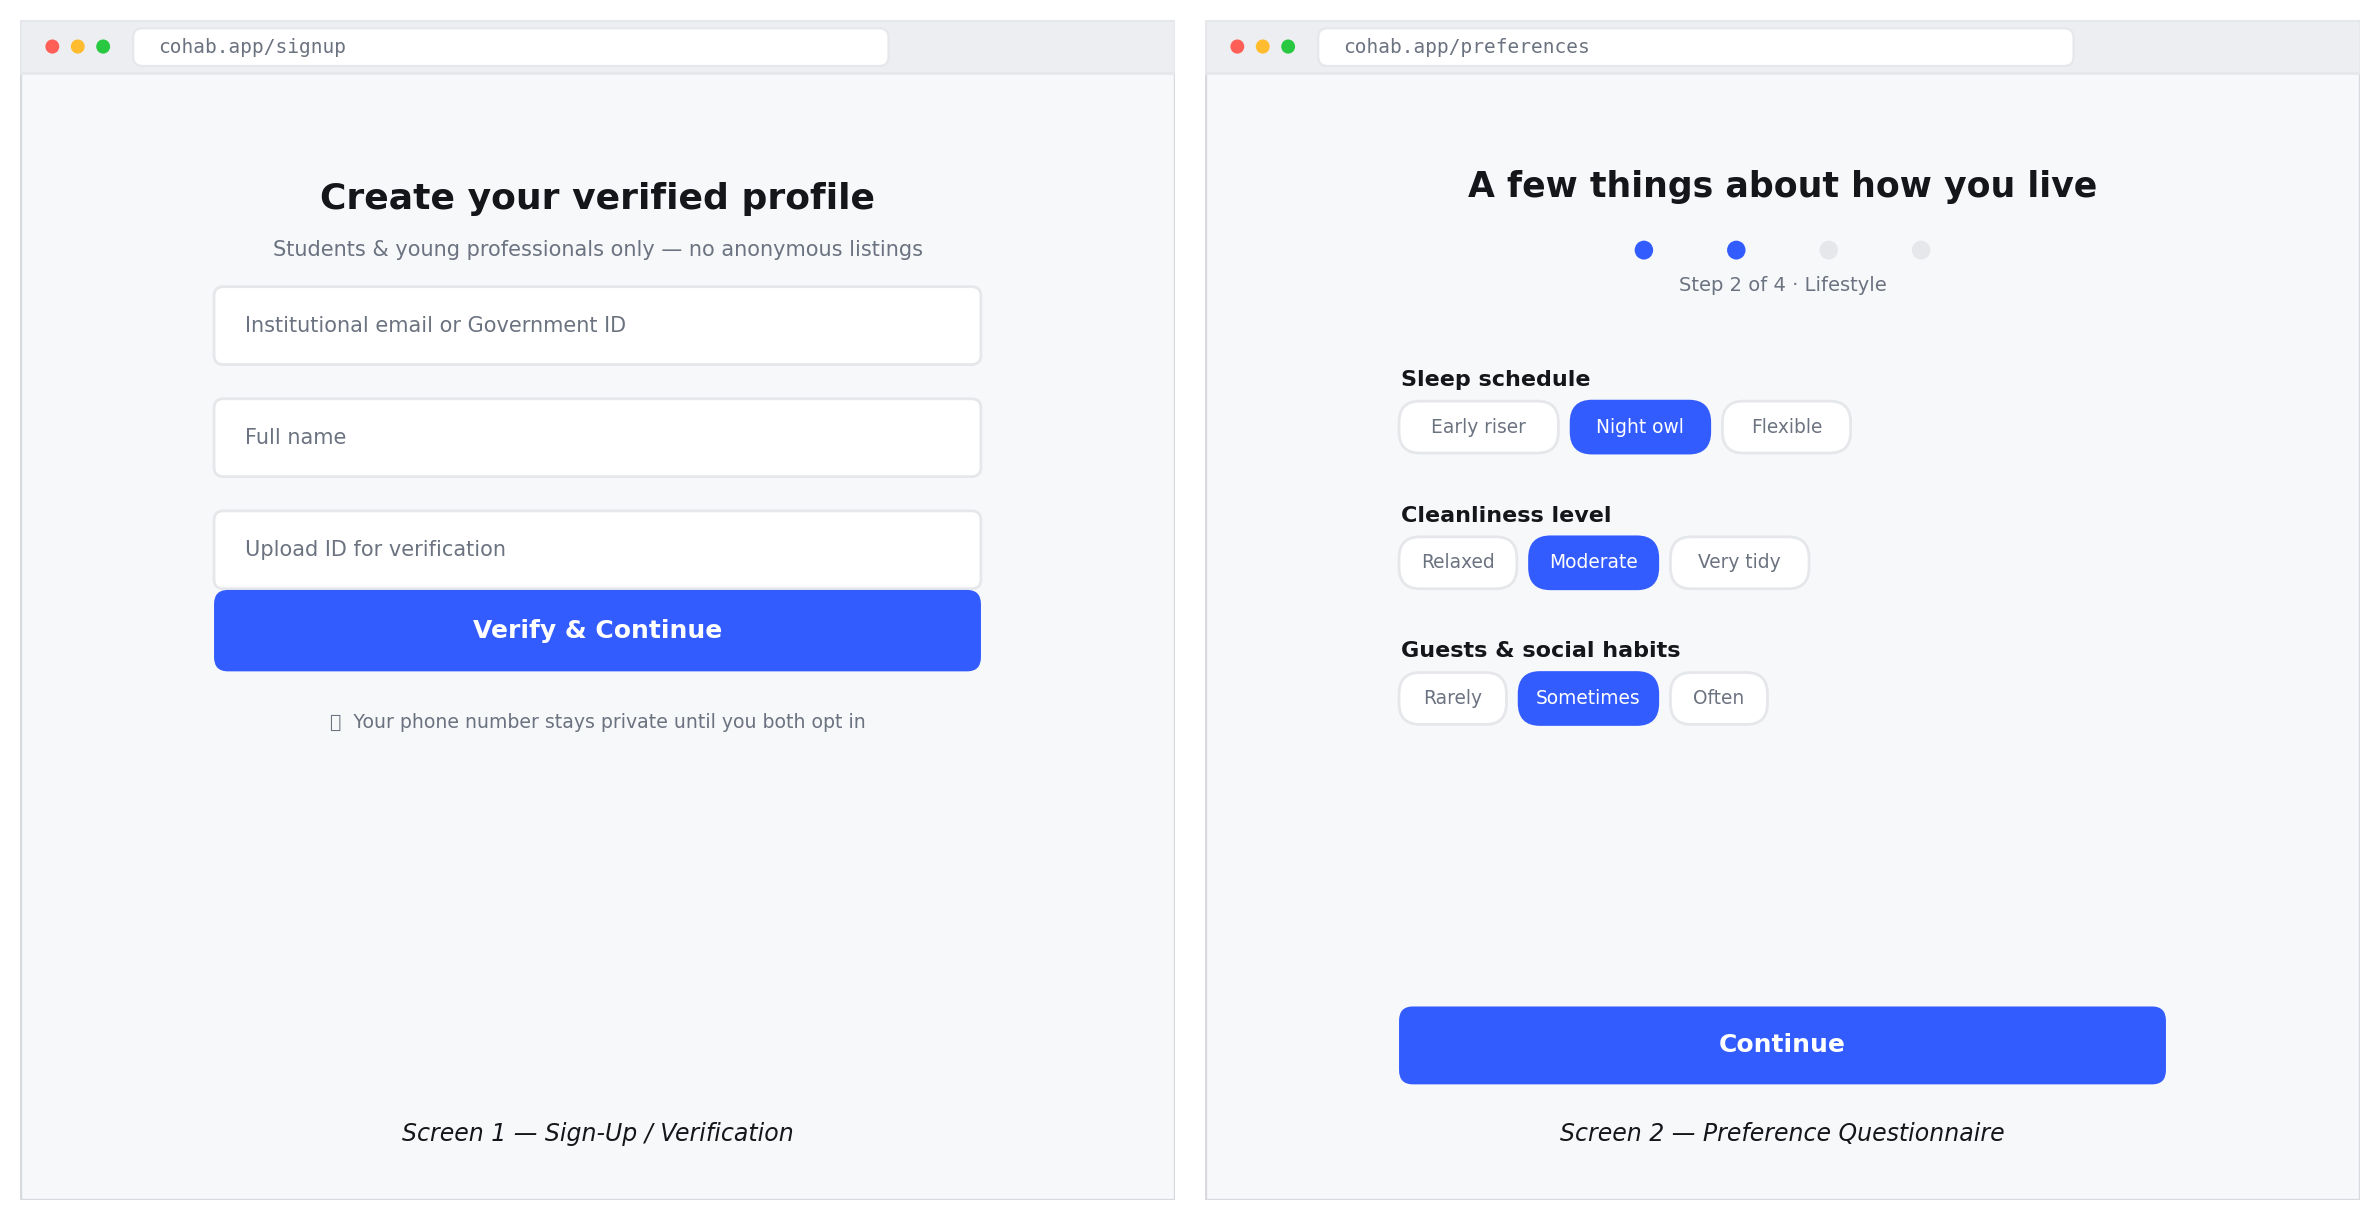
\includegraphics[width=1.0\textwidth]{image12.png}
    \caption{Wireframes -- Sign-Up and Preference Questionnaire Screens}
    \label{fig:11.1}
\end{figure}

\begin{figure}[htbp]
    \centering
    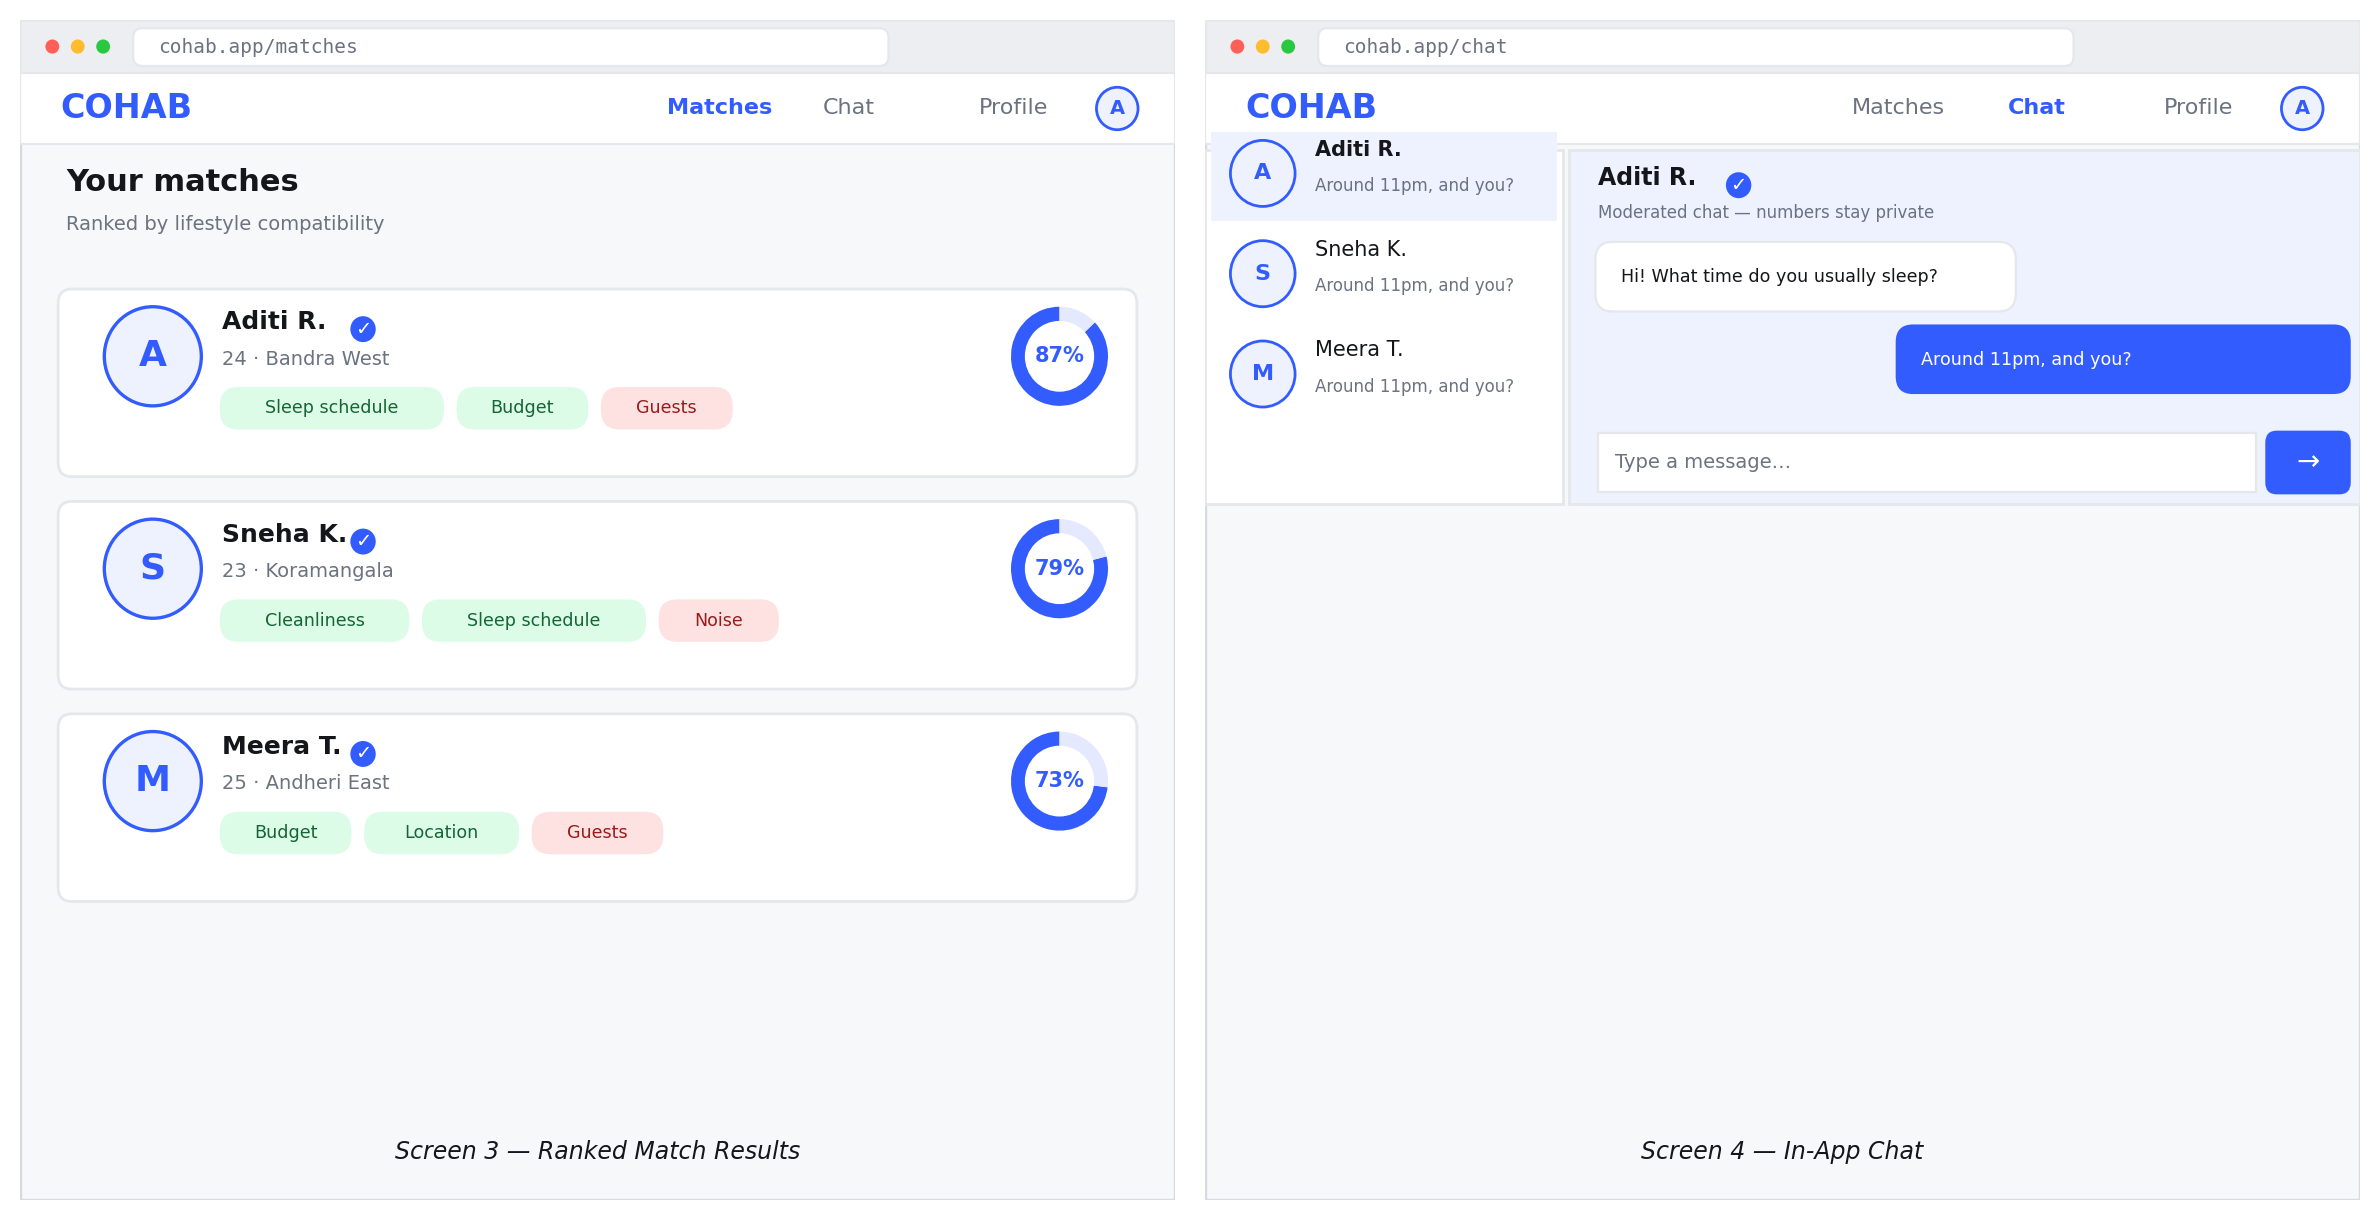
\includegraphics[width=1.0\textwidth]{image13.png}
    \caption{Wireframes -- Match Results and In-App Chat Screens}
    \label{fig:11.2}
\end{figure}

\begin{figure}[htbp]
    \centering
    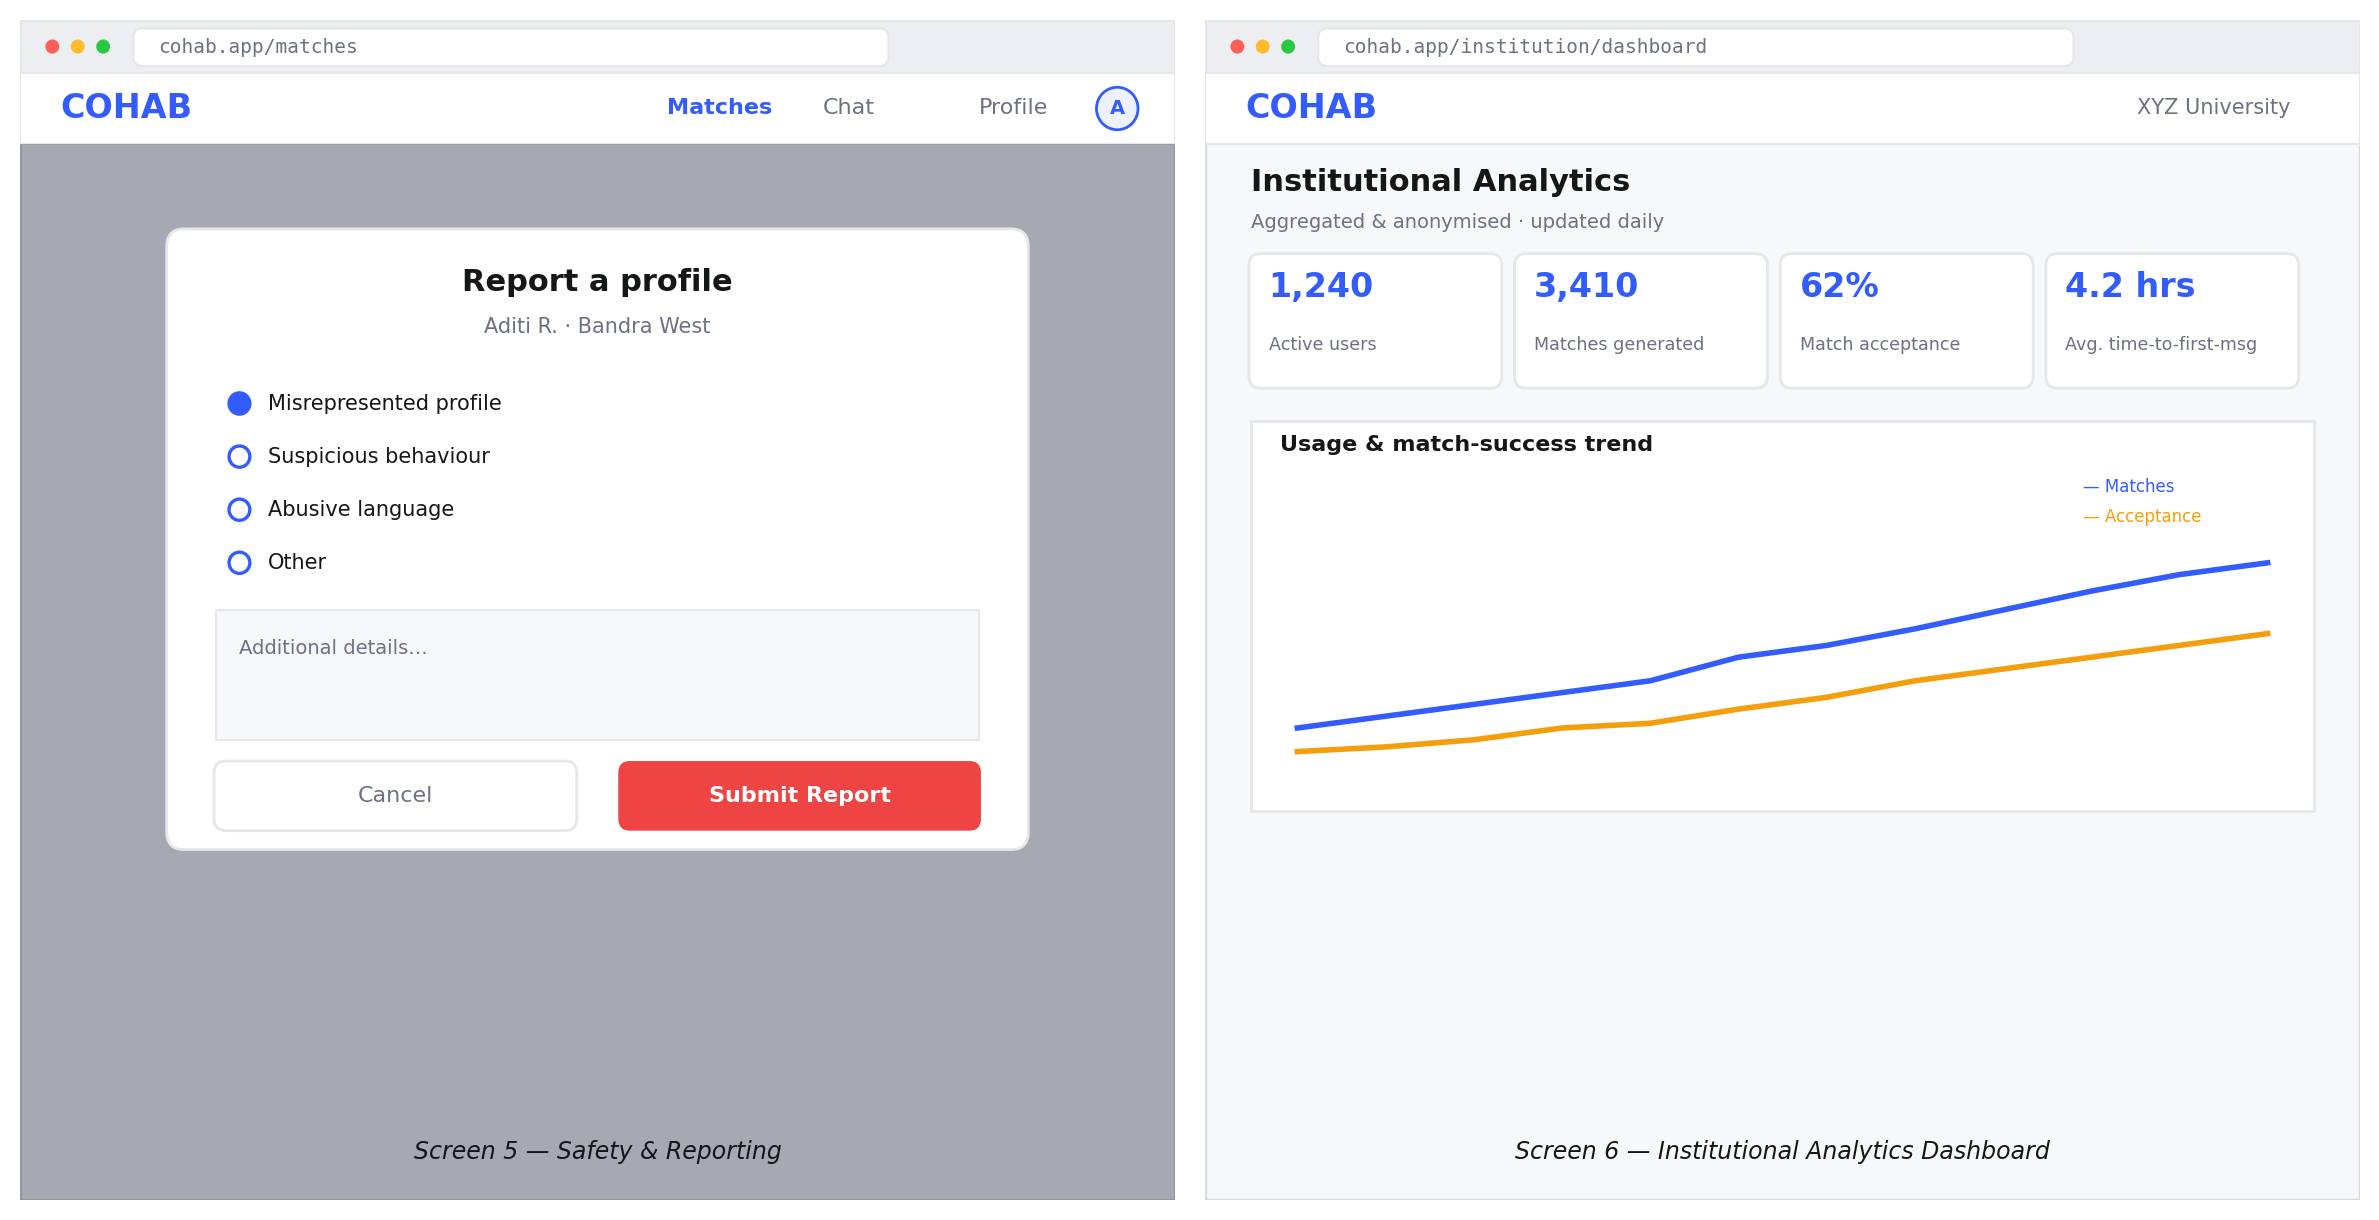
\includegraphics[width=1.0\textwidth]{image14.png}
    \caption{Wireframes -- Safety Reporting and Institutional Analytics Screens}
    \label{fig:11.3}
\end{figure}






% ==================================================================
\chapter{Project Schedule (Gantt Chart)}

\section{Trimester Timeline}

The Gantt chart below aligns the project workstreams with the Even Trimester 2026--2027 course-plan weeks, extending the tentative 12-week plan from the Synopsis into the full 16-week trimester structure to also cover deployment and final reporting. Figures \ref{fig:12.1} and \ref{fig:12.2} are generated from a single activity table, so the bar chart and the network analysis describe the same schedule by construction.

\vspace{6mm}

\begin{figure}[htbp]
    \centering
    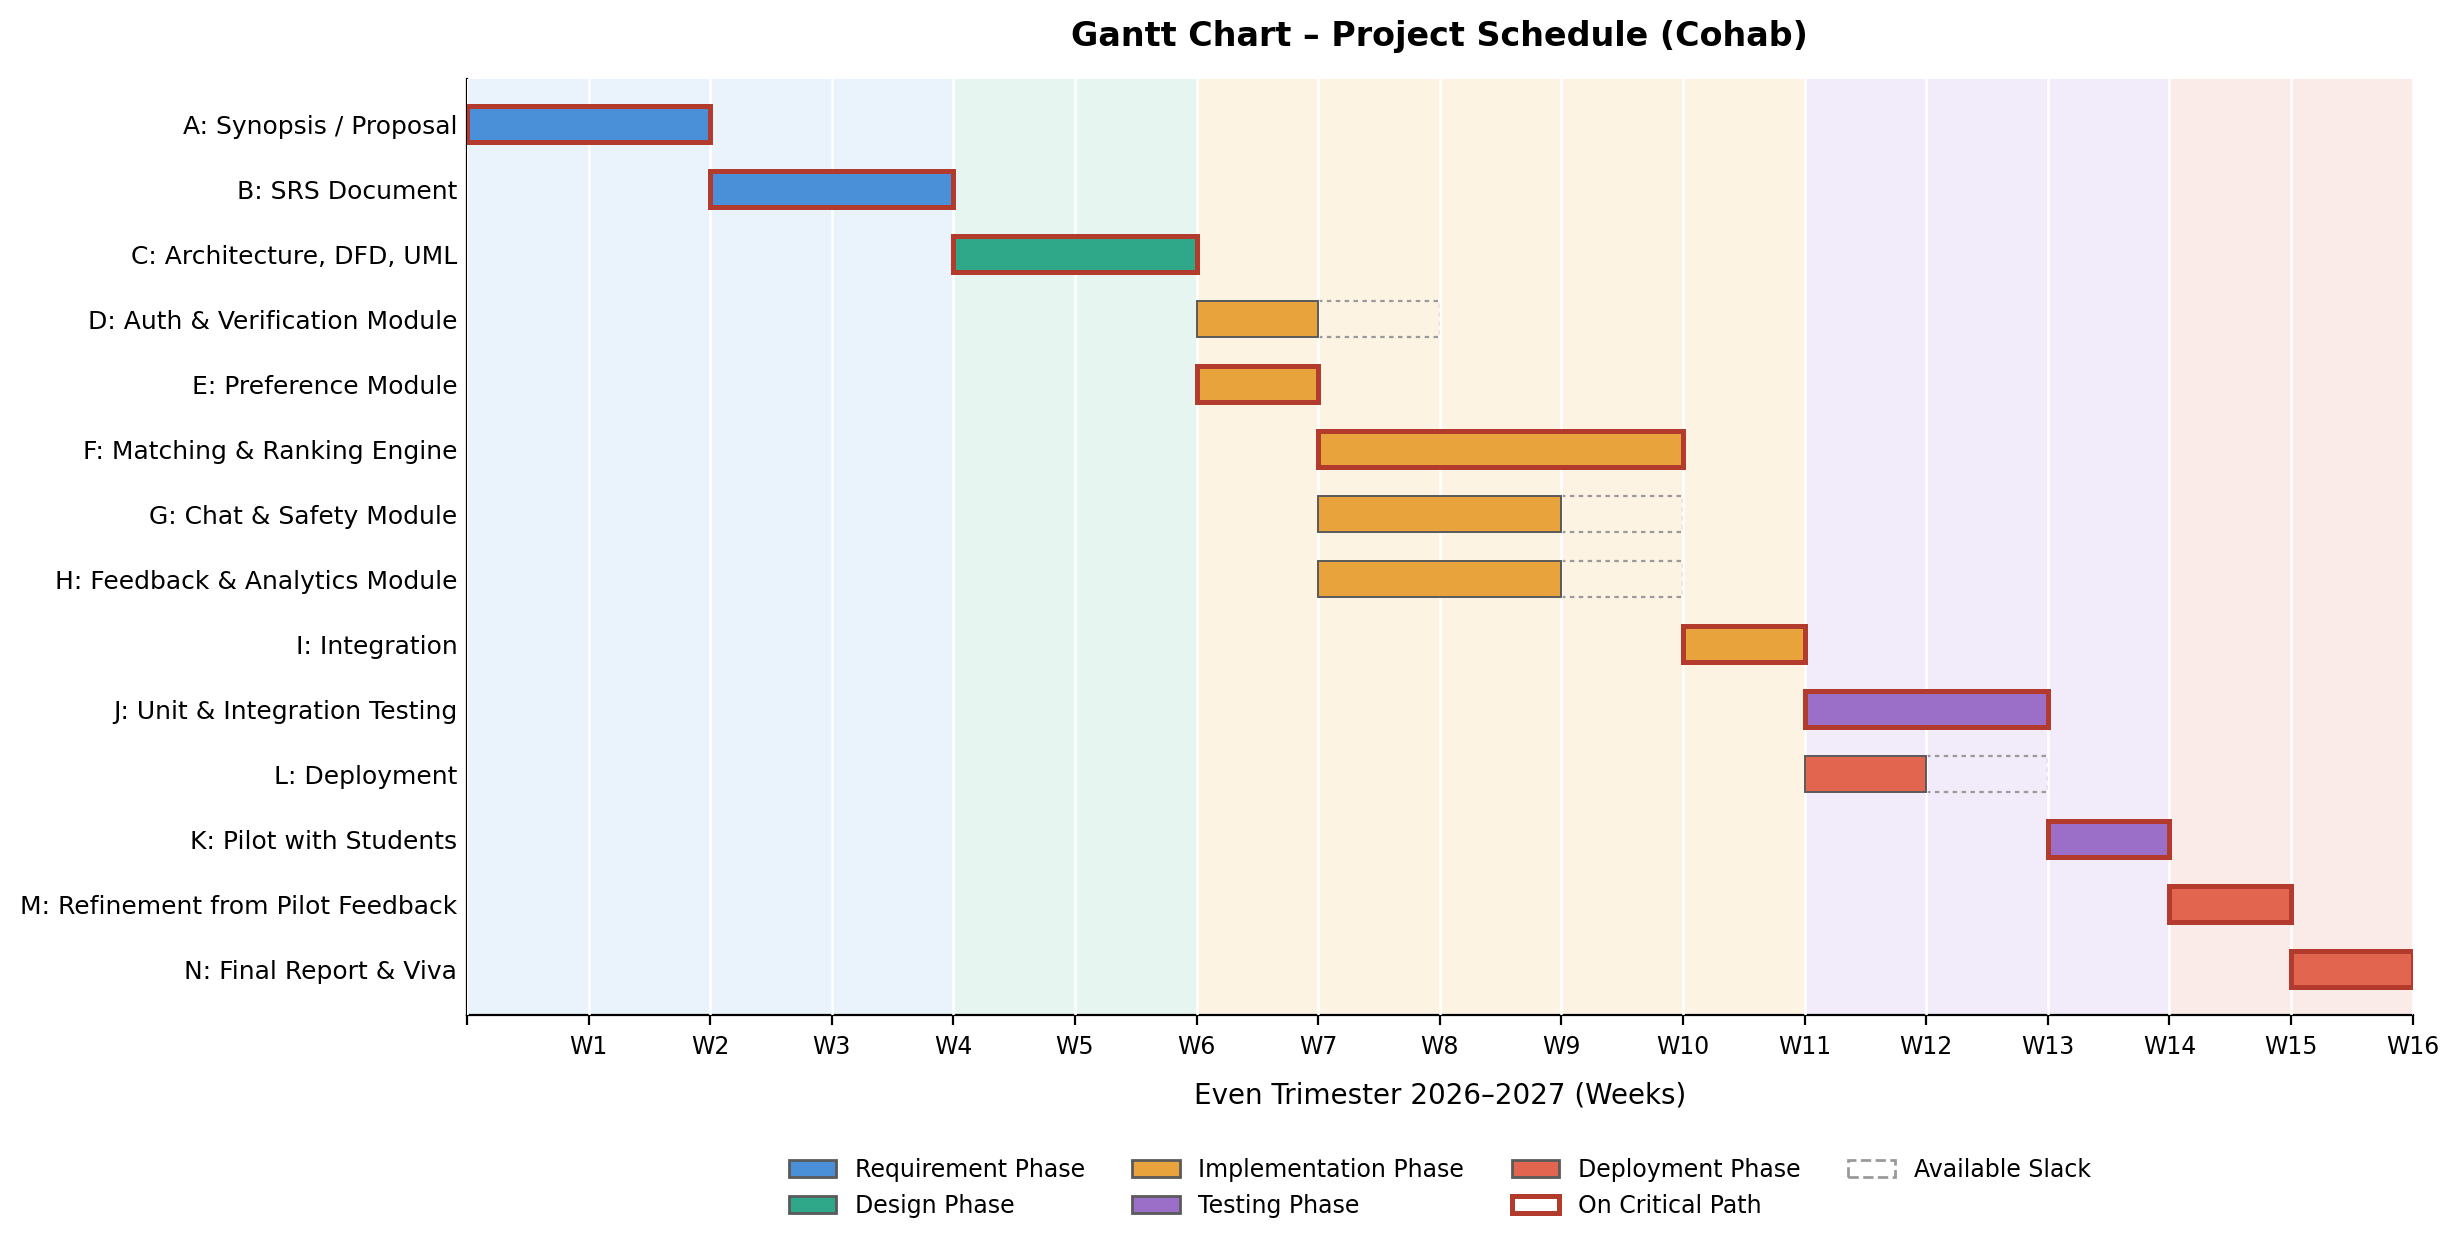
\includegraphics[width=1.0\textwidth]{images/image15.png}
    \caption{Gantt Chart -- Project Schedule}
    \label{fig:12.1}
\end{figure}

Figure \ref{fig:12.1} presents the planned project timeline for Cohab across the academic trimester. Weeks 1--2 cover the Synopsis/Proposal, and weeks 3--4 the SRS document produced during Requirement Analysis. Weeks 5--6 correspond to the current System Design phase --- architecture, DFDs, UML diagrams, and this document. Weeks 7--10 cover implementation, proceeding module by module: the authentication and verification module and the preference module in week 7, then the matching and ranking engine across weeks 8--10 running in parallel with the chat and safety module and the feedback and analytics module. Week 11 is integration. Weeks 12--13 cover unit and integration testing, with deployment to the pilot environment in week 12 so that the environment is ready when testing concludes. Week 14 is the student pilot, week 15 covers refinement from pilot feedback, and week 16 the final report and viva. This incremental strategy ensures timely completion of deliverables while allowing continuous integration and validation of individual modules.

The dashed extensions on the bars for the Auth \& Verification, Chat \& Safety, Feedback \& Analytics and Deployment activities show the float available to each: these activities may overrun by the indicated amount without moving the project end date.

\vspace{8mm}

\section{PERT / CPM Network Diagram}

To identify which activities directly drive the overall project duration, the same fourteen work packages from Figure \ref{fig:12.1} are modelled as a PERT (Program Evaluation and Review Technique) activity-on-node network and analysed using the Critical Path Method (CPM). Each node records the activity's duration together with its Earliest Start (ES), Earliest Finish (EF), Latest Start (LS), Latest Finish (LF), and Slack (LS $-$ ES). Times are expressed in weeks elapsed since the start of the trimester, so ES $= 0$ denotes the beginning of Week 1 and EF $= 16$ the end of Week 16.

\begin{figure}[htbp]
    \centering
    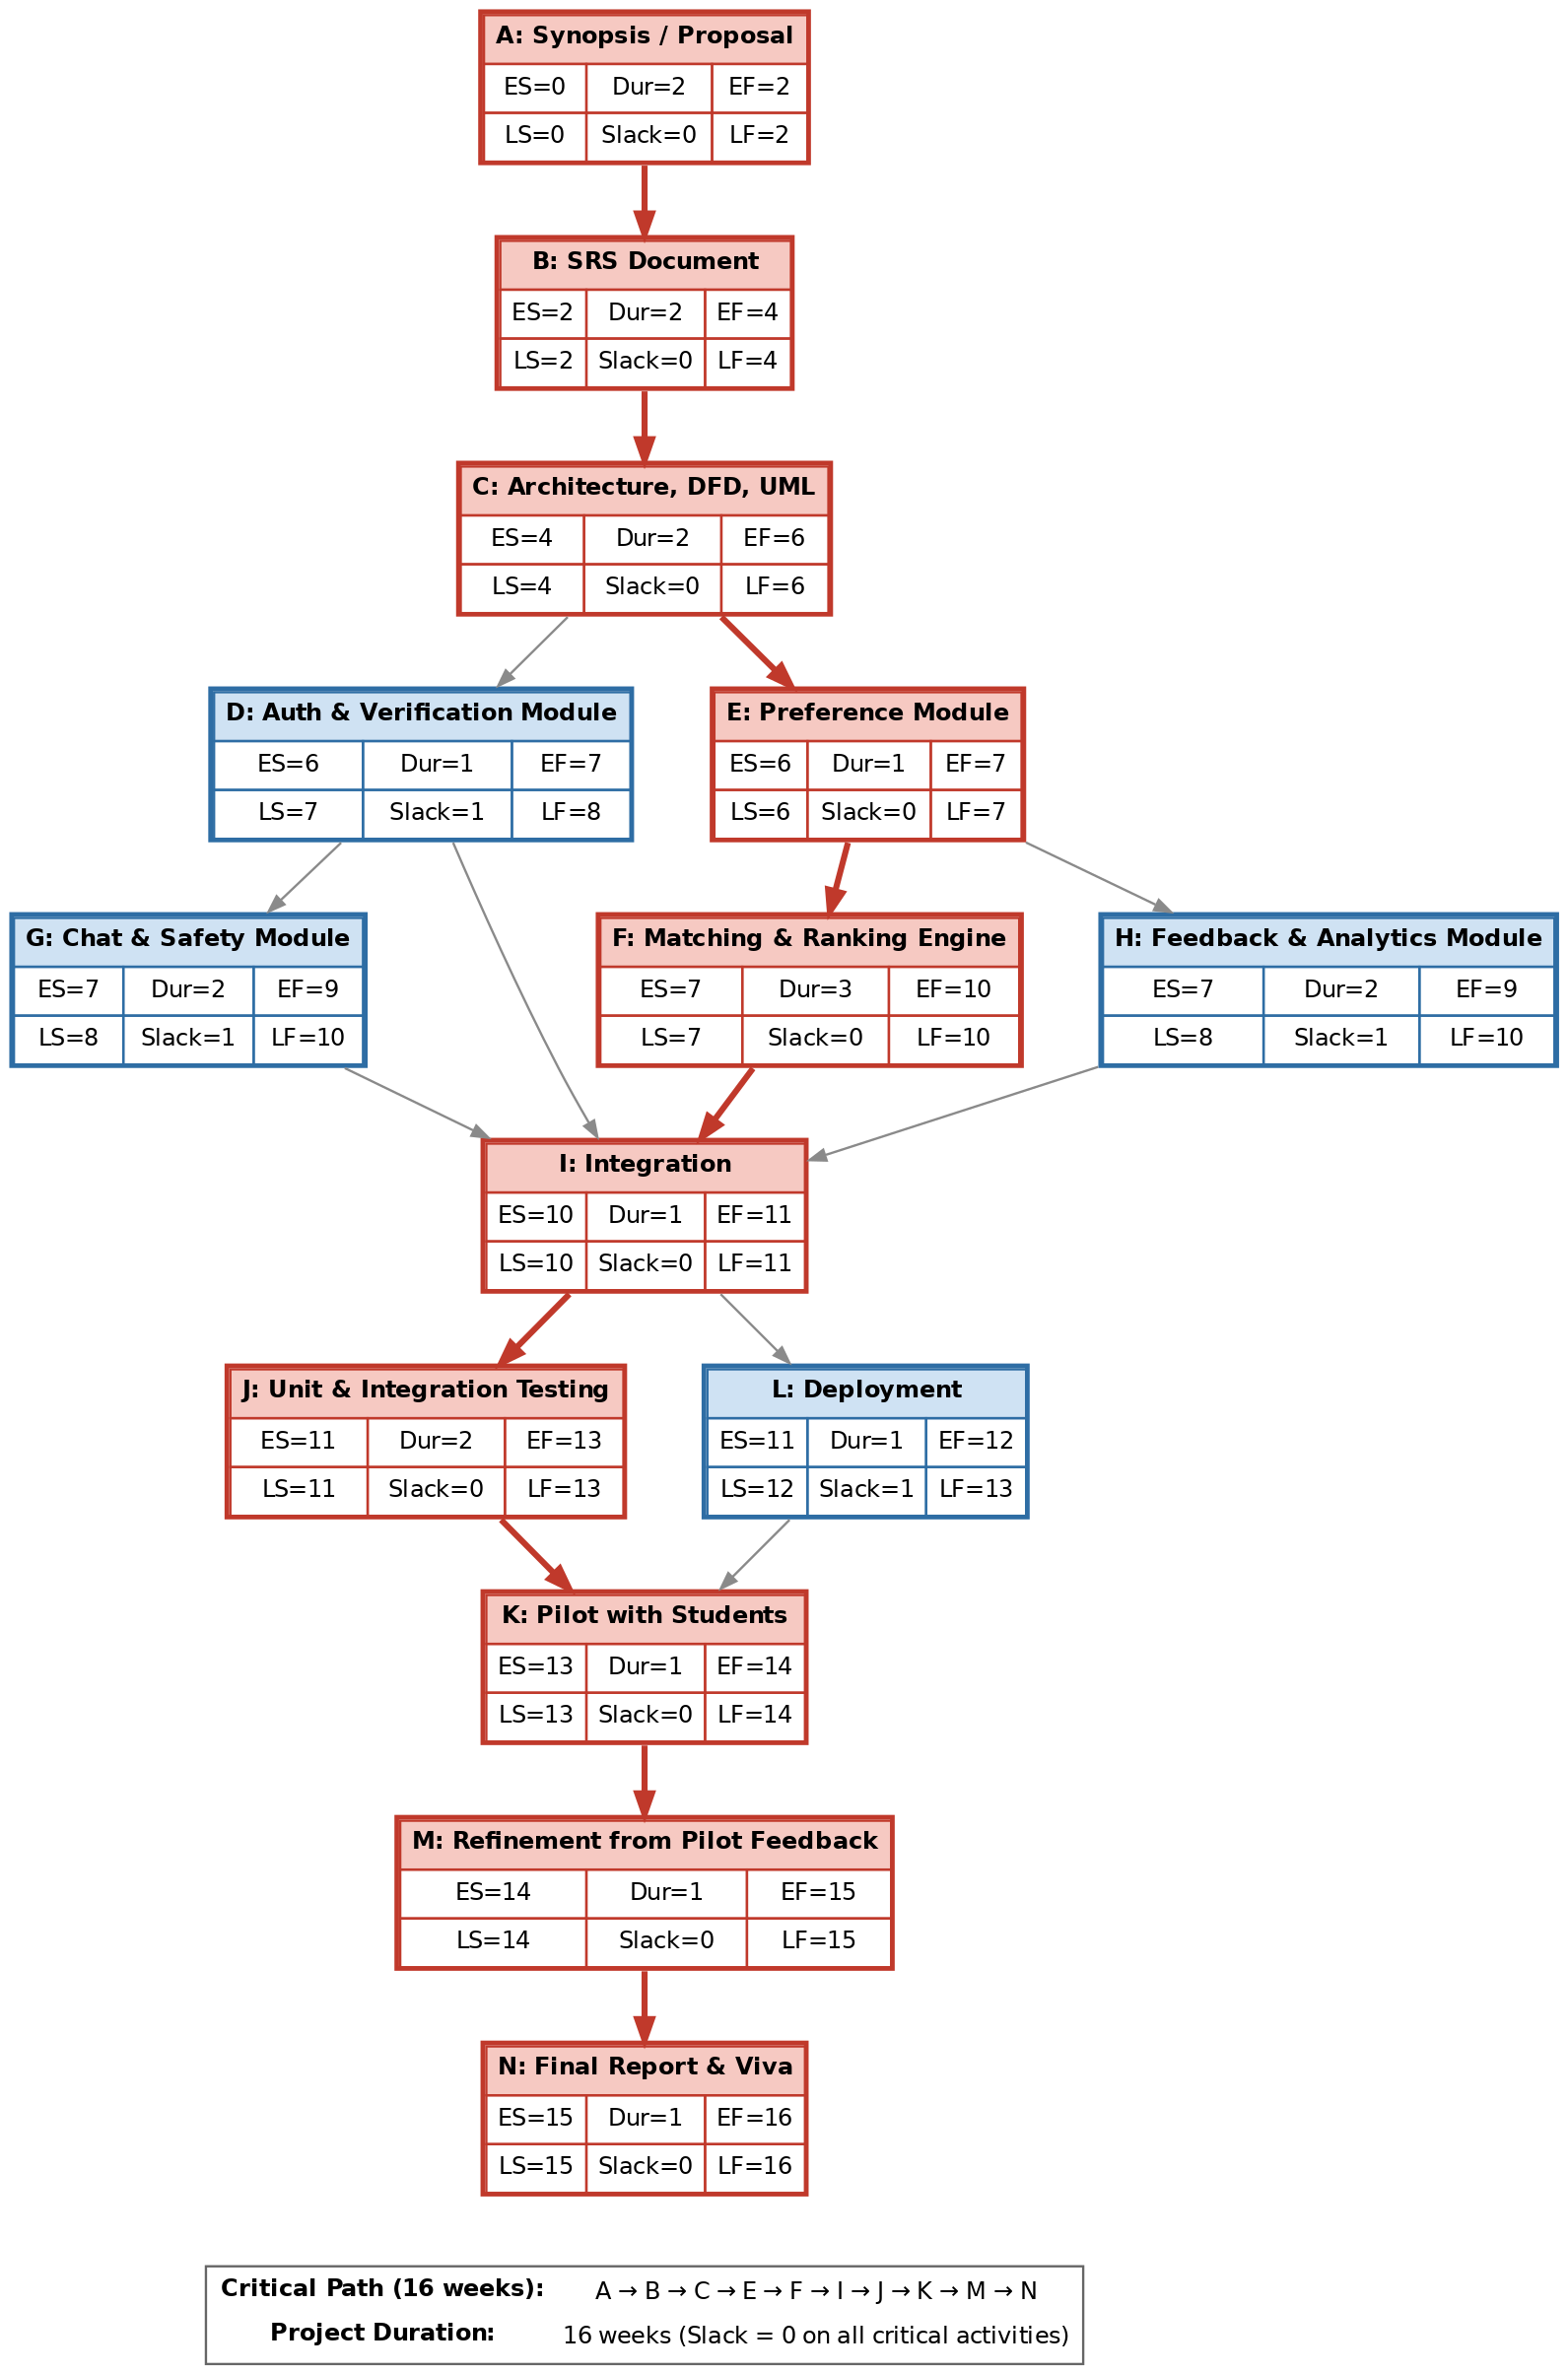
\includegraphics[height=0.8\textheight]{images/image16.png}
    \caption{PERT / CPM Network Diagram with Critical Path Highlighted}
    \label{fig:12.2}
\end{figure}

The activities outlined in red in Figure \ref{fig:12.2} form the critical path: Synopsis/Proposal $\rightarrow$ SRS Document $\rightarrow$ Architecture/DFD/UML $\rightarrow$ Preference Module $\rightarrow$ Matching \& Ranking Engine $\rightarrow$ Integration $\rightarrow$ Unit \& Integration Testing $\rightarrow$ Pilot with Students $\rightarrow$ Refinement from Pilot Feedback $\rightarrow$ Final Report \& Viva. Summing the durations along this chain gives $2+2+2+1+3+1+2+1+1+1 = 16$ weeks, which matches the trimester length and the span of the Gantt chart in Figure \ref{fig:12.1}. These activities have zero slack, meaning any delay to one of them delays the entire project; they therefore warrant the closest schedule monitoring.

Four activities carry float and are not on the critical path: the Auth \& Verification Module, the Chat \& Safety Module, the Feedback \& Analytics Module (1 week each), and Deployment (1 week). The three module activities run in parallel with the critical Preference Module $\rightarrow$ Matching \& Ranking Engine sequence and are re-synchronised at Integration, so minor delays to them can be absorbed without shifting the overall timeline. Deployment carries float because it is scheduled to run alongside testing rather than after it: the pilot environment is prepared while the test suite is still executing, and only the pilot itself depends on both being complete.

The scheduling implication is that the Matching \& Ranking Engine is the single activity most likely to determine whether the project finishes on time. It has the longest duration of any implementation activity, it sits on the critical path, and it depends on the Preference Module immediately upstream of it. Any slippage in the preference questionnaire propagates directly into it with no buffer.

% ==================================================================
\chapter{Conclusion}

This System Design Document translates the requirements defined in the SRS into a concrete, implementable design: a layered architecture separating presentation, gateway, business logic, AI/ML, and persistence concerns; a component view of the core business-logic modules with server-side orchestration; data flow across five major processes; a use-case model covering every stakeholder interaction; a normalised ERD with an accompanying data dictionary and explicit integrity constraints; a modular class design in which the weight-refinement loop is closed through a versioned registry rather than a circular dependency; an activity diagram capturing the full matching-to-chat workflow, supported by explicit state models for the match and report lifecycles; a representative sequence diagram for the core matching flow; a two-stage algorithm design separating non-negotiable eligibility constraints from graded, explainable preference scoring, with a planned Gradient-Boosted Tree ranking upgrade once outcome data accumulates and an optional stable-roommates extension for institutional batch allocation --- together with their supporting data structures; a security, privacy and DPDP compliance design; an evaluation design fixing success criteria in advance of the pilot; interface wireframes for the six key screens; and a Gantt chart and PERT/CPM network, generated from a common activity table, aligning development with the 16-week trimester timeline.

Three design decisions in particular distinguish this version from a direct translation of the SRS. Separating hard constraints from soft preferences prevents the system from ever recommending a candidate who is infeasible in practice, which no adjustment of weights within a single scoring function could achieve. Versioning the scoring weights makes explanations reproducible, without which the Explainability requirement would hold only at the moment a score was first shown. Identifying the correct algorithm for the non-bipartite stable roommates problem, and acknowledging that such a matching need not exist, ensures the batch-allocation extension is specified on a sound basis rather than on an algorithm defined for a different problem.

This design forms the basis for the subsequent Implementation and Testing phases of the project.

\vspace{2em}
\end{document}
